\documentclass[11pt]{beamer}
%\usetheme{Juelich}
\usepackage{beamertheme/beamerthemeJuelich}

\usepackage{appendixnumberbeamer}
\usepackage{epstopdf}
\setbeamertemplate{footer element1}[logo]{logos/BUW_Logo-schwarz}
\setbeamertemplate{frame number}[full]

\usepackage{subcaption} % subfigure
\usepackage{tcolorbox}

\usepackage{booktabs} % midrule
\usepackage{colortbl} % rowcolor
\usepackage{multirow}

\usepackage{xcolor}
\usepackage{pgfplots}
\usepackage{femtikz}
\usetikzlibrary{shapes,arrows,positioning}
\usepgfplotslibrary{colorbrewer}
\usepgfplotslibrary{groupplots}

\pgfplotsset{select coords between index/.style 2 args={
    x filter/.code={
      \ifnum\coordindex<#1\def\pgfmathresult{}\fi
      \ifnum\coordindex>#2\def\pgfmathresult{}\fi
    }
}}

\usepackage{isomath}
\newcommand{\h}{\textit{h}}
\newcommand{\p}{\textit{p}}
\newcommand{\hp}{\textit{hp}}

\newcommand{\dealii}{\texttt{deal.II}}
\newcommand{\pforest}{\texttt{p4est}}
\newcommand{\petsc}{\texttt{PETSc}}
\newcommand{\trilinos}{\texttt{Trilinos}}
\newcommand{\epetra}{\texttt{Epetra}}
\newcommand{\aztecoo}{\texttt{AztecOO}}
\newcommand{\ml}{\texttt{ML}}
\newcommand{\xsdk}{\texttt{xSDK}}

\newcommand{\opencascade}{\texttt{OpenCASCADE}}
\newcommand{\opensalome}{\texttt{OpenSALOME}}
\newcommand{\fftw}{\texttt{FFTW}}
\newcommand{\mofem}{\texttt{MoFEM}}
\newcommand{\phg}{\texttt{PHG}}
\newcommand{\phaml}{\texttt{PHAML}}


\usepackage[backend=biber, style=authoryear]{biblatex}
\addbibresource{misc/bibliography.bib}



\author{Marc Fehling~~\vrule width0.3pt~~m.fehling@fz-juelich.de}
\title{Algorithms for massively parallel generic hp-adaptive FEM}
\subtitle{\vspace{-1em}}
\titlegraphic{
  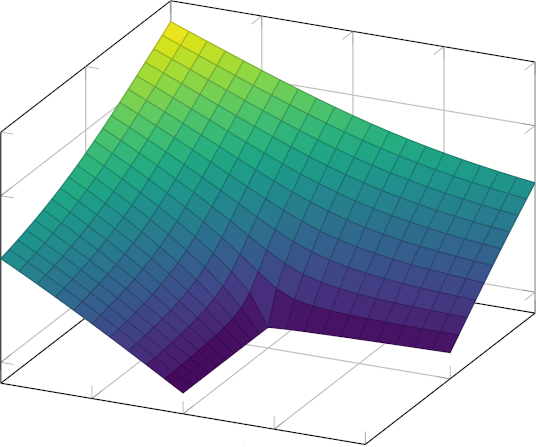
\includegraphics[height=0.37\paperheight]{figures/corner_447px.png}
  \hspace{.1em}
  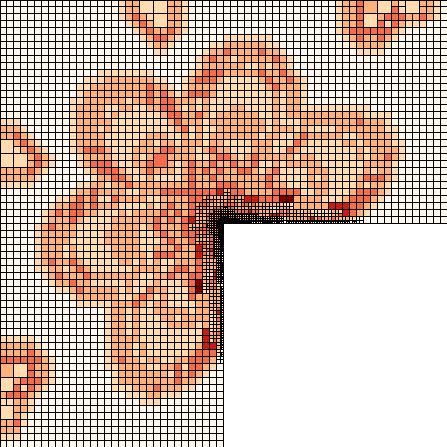
\includegraphics[height=0.37\paperheight]{figures/corner-fedegrees-legendre-05_447px.png}
  \hspace{.1em}
  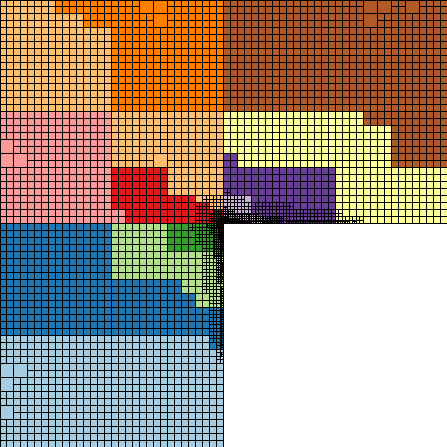
\includegraphics[height=0.37\paperheight]{figures/corner-subdomains-legendre-05_447px.png}
}
\date{June 05, 2020}
%\institute{Institute for Advanced Simulation (IAS)}



\begin{document}

\maketitle

\begin{frame}
\frametitle{Table of contents}
\tableofcontents
\end{frame}

\chapter{Introduction}
\label{ch:introduction}

\todo{Introduction:}
\begin{itemize}
  \item Need for new computational methods (adaptive)
  \item Statistics on usage of FDS? (literatur aus bennis diss?)
  
  \item Latest catastrophes: tower, Düsseldorf
  \item ... help to .. catastrophes by giving hints on placements of safety measures.
\end{itemize}

Recent advancements in computer technology allows us to solve problems with billions of unknowns. However, raw computing power does not mean we can use it without further ado. The keys to efficiency are algorithms that exploit the hardware structure and focus resources on critical operations.

For currently common multi-processor systems, algorithms for parallelization need to be supplied . These methods depend on the hardware architecture, and especially large-scale supercomputers with distributed memory access benefit from this method.

Lots of \glspl{api} exist for these purposes, that allow users to take opportunity of already implemented ideas.

For machines with shared memory access, \glsdesc{openmp}\glsunset{openmp} \parencite{openmp50} and \glsdesc{tbb}\glsunset{tbb} \parencite{tbb2018} with its work stealing policy are the most prominent approaches. IF architecture is distributed on nodes and thus have distributed memory access, the \glsdesc{mpi}\glsunset{mpi} \parencite{mpi31} will be used. A combination of both is possbile.

Further, recently streaming multiprocessor architecture have become more and more interest, that work on graphic accelerator cards (GPUS). \glsdesc{openacc}\glsunset{openacc} \parencite{openacc27} or nVidia's \glsdesc{cuda}\glsunset{cuda} \parencite{cuda10} can be used for that.

On the other hand, . adaptive

A combinatation of both hardware and .. software driven algorithms can be supplied. However, their combination is not trivial. 

"MPI remains the dominant library for production programming on large scale distributed memory machines."

Some typeof hardware-related 
To name a few, Hardware-related algorithms are parallelization, vectorization and limiting memory access, since it. In terms 


guarantee the full usage of all available resources. The key to use those ausnutzen fully are efficient algorithms that either fit to the hardware or distribute resources on computing intensive operations.

However, the key to use these structures efficientis to , and not computing power alone; (Erst) the combination with algorithms that use these structure efficiently offers a massive potential to reduce 




Some of them

parallelization, vectorization, limit memory access. adaptive methods

parallelization depending on hardware architecture: MPI for distributed memory, OpenMP for shared memory, OpenACC or nVidia CUDA for streaming multiprocessors on e.g. GPUs

adaptive methods to focus .


Each algorithm . The combination of both is more or less trivial.
On supercomputers
This thesis presents the combination of both parallelization on distributed hardware architecture, and hp-adaptive methods.

For spatial discretizations we use . The \gls{fem}


This dissertation is not meant to be an in-depth guide for the creation of \gls{fem} software. We would rather like to emphasize on the basic ideas for parallel hp-adaptive \gls{fem} and point out programming challenges. We will provide an example implementation in the \dealii{} library, so that the reader is able to either embed our findings into his own \gls{fem} code or use the \dealii{} implementation right away.
\section{hp-adaptive methods}





\begin{frame}
\frametitle{Table of contents}

\tableofcontents[currentsection]
\end{frame}





\subsection{Finite Element Method}





\begin{frame}
\frametitle{Finite element method}

\begin{minipage}{.59\textwidth}
  \begin{itemize}
  \item Shape functions form nodal basis
    \begin{align*}
    \varphi_i(x_j) = \delta_{ij} =
    \begin{cases}
    1 & \text{for} ~ i=j \\
    0 & \text{for} ~ i \neq j
    \end{cases}
    \end{align*}
  \item $Q_p$ elements from Lagrange interpolation with degree $p$
  \end{itemize}
  
  \vspace{1em}
  
  \begin{itemize}
  \item Finite element approximation is linear combination of shape functions
    \begin{align*}
    u_{hp}(x) = \sum_i \, u_i \, \varphi_i(x)
    \end{align*}
  \item Coefficients $u_i$ are degrees of freedom
  \end{itemize}
\end{minipage}
\hfill
\begin{minipage}{.4\textwidth}
  \vspace{-1em}
  
  \begin{figure}
  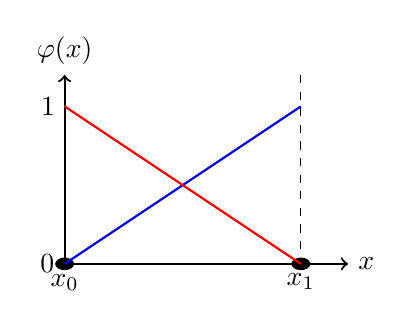
\begin{tikzpicture}[scale=2, xscale=1.5]
  % Draw axes
  \draw [<->,thick] (0,0) node [below] {$x_0$} node[left] {0}
  (0,1.2) node (yaxis) [above] {$\varphi(x)$}
  |- (1.2,0) node (xaxis) [right] {$x$};
  
  % Draw dashed
  \draw [dashed] (1,1.2) -- (1,0) node [below] {$x_1$};
  
  % Draw nodes
  \foreach \x in {0,1} {
    \fill (\x,0) circle (.04cm);
    %\fill (\x,1) circle (.04cm);
  }
  \node[left] at (0,1) {1};
  
  % Draw functions
  \draw[thick,color=blue,domain=0:1] plot (\x,{\x});
  \draw[thick,color=red,domain=0:1] plot (\x,{1-\x});
  \end{tikzpicture}
  \vspace{-0.8em}
  \caption{$Q_1$ element}
  \end{figure}
  
  \vspace{-2.5em}
  
  \begin{figure}
  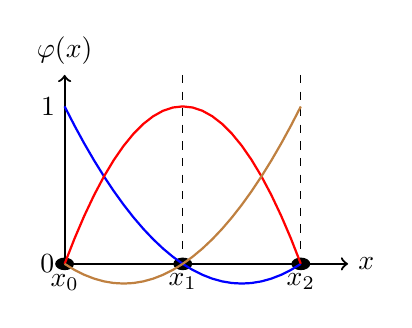
\begin{tikzpicture}[scale=2, xscale=1.5]
  % Draw axes
  \draw [<->,thick] (0,0) node [below] {$x_0$} node[left] {0}
  (0,1.2) node (yaxis) [above] {$\varphi(x)$}
  |- (1.2,0) node (xaxis) [right] {$x$};
  
  % Draw dashed
  \draw [dashed] (0.5,1.2) -- (0.5,0) node [below] {$x_1$};
  \draw [dashed] (1,1.2) -- (1,0) node [below] {$x_2$};
  
  % Draw nodes
  \foreach \x in {0,0.5,1} {
    \fill (\x,0) circle (.04cm);
    %\fill (\x,1) circle (.04cm);
  }
  \node[left] at (0,1) {1};
  
  % Draw functions
  \draw[thick,color=blue,domain=0:1] plot (\x,{2*\x*\x - 3*\x + 1});
  \draw[thick,color=red,domain=0:1] plot (\x,{(-4)*\x*\x + 4*\x});
  \draw[thick,color=brown,domain=0:1] plot (\x,{2*\x*\x - \x});
  \end{tikzpicture}
  \vspace{-0.8em}
  \caption{$Q_2$ element}
  \end{figure}
\end{minipage}
\end{frame}





\subsection{Adaptive methods}





\begin{frame}
\frametitle{Adaptive methods}

\begin{itemize}
\item Focus computational resources on areas of interest
\item Align simulation resolution with complexity of current solution
\end{itemize}

\vfill{}

\begin{itemize}
\item Finite Element Method (FEM) provides two different possibilities:
\begin{tabular}{lll}
  \textbf{\h}-adaptation: & dynamic cell sizes & good for irregular solutions \\
  \textbf{\p}-adaptation: & dynamic function spaces & good for smooth solutions
\end{tabular}
\item Combination of both possible
\end{itemize}

\vfill{}

\begin{minipage}{.49\textwidth}
  \begin{figure}
  \begin{tikzpicture}[scale=2.2]
  \def\Length{0.5}
  \def\Radius{0.03}
  
  \LagrangeCell{-2*\Length}{0}{2*\Length}{\Radius}{2}
  {{,,,,,,,,}};
  
  % remove face node which becomes a hanging node on a vertex
  \draw[fill=white,draw=white] (0,\Length-\Radius) rectangle (-\Radius,\Length+\Radius);
  
  \LagrangeCell{0}{0}{\Length}{\Radius}{2}
  {{,,,,,,,,}};
  \LagrangeCell{\Length}{0}{\Length}{\Radius}{2}
  {{,,,,,,,,}};
  \LagrangeCell{0}{\Length}{\Length}{\Radius}{2}
  {{,,,,,,,,}};
  \LagrangeCell{\Length}{\Length}{\Length}{\Radius}{2}
  {{,,,,,,,,}};
  \end{tikzpicture}
  \caption{\h-adaptivity}
  \end{figure}
\end{minipage}
\begin{minipage}{.49\textwidth}
  \begin{figure}
  \begin{tikzpicture}[scale=2.2]
  \def\Length{1}
  \def\Radius{0.03}
  
  \LagrangeCell{0}{0}{\Length}{\Radius}{2}
  {{,,,,,,,,}};
  \LagrangeCell{\Length}{0}{\Length}{\Radius}{4}
  {{,,,,,,,,,,,,,,,,,,,,,,,,}};
  \end{tikzpicture}
  \caption{\p-adaptivity}
  \end{figure}
\end{minipage}
\end{frame}





\begin{frame}
\frametitle{Adaptation criteria}

\begin{itemize}
\item \textbf{Which} cells to adapt?
\item \textbf{How} to adapt? \h/\p?
\end{itemize}

\pause
\vfill{}

\begin{itemize}
\item Manual adaptation
\item Automatic adaptation
  \begin{itemize}
  \item Criterion to indicate adaptation
  \item General approach -OR- tied to the problem
  \end{itemize}
\end{itemize}

\pause
\vfill{}

\begin{itemize}
\item Automatic \hp-decision strategies discussed in the dissertation
  \begin{enumerate}
  \item Error prediction based on refinement history \newline \parencite{melenk2001}
  \item Smoothness estimation by decay of Fourier coefficients \newline \parencite{bangerth2009}
  \item Smoothness estimation by decay of Legendre coefficients \newline \parencite{mavriplis1994}
  \end{enumerate}
\end{itemize}
\end{frame}





\subsection{Example: Laplace equation}





\begin{frame}
\frametitle{Example: Reentrant corner}

\begin{minipage}{.47\textwidth}
\begin{itemize}
  \item Singularity at reentrant corners for elliptic problems
  \item L-shaped domain:
    \begin{align*}
    \Omega = [-1,1]^2 \setminus \left([0,1]\!\times\![-1,0]\right)
    \end{align*}
  \item Manufactured Laplace problem
    \begin{align*}
    - \nabla^2 u &= 0 \qquad\text{on}\quad \Omega \\
    u &= \bar{u} \qquad\text{on}\quad \partial\Omega \\[.5em]
    \bar{u} &= r^{2/3} \, \sin\left(2/3 ~ \varphi\right) \\
    \|\nabla \bar{u}\| &= r^{-1/3}
    \end{align*}
\end{itemize}
\end{minipage}
\hfill{}
\begin{minipage}{.51\textwidth}
  \begin{figure}
  \resizebox{\textwidth}{!}{
    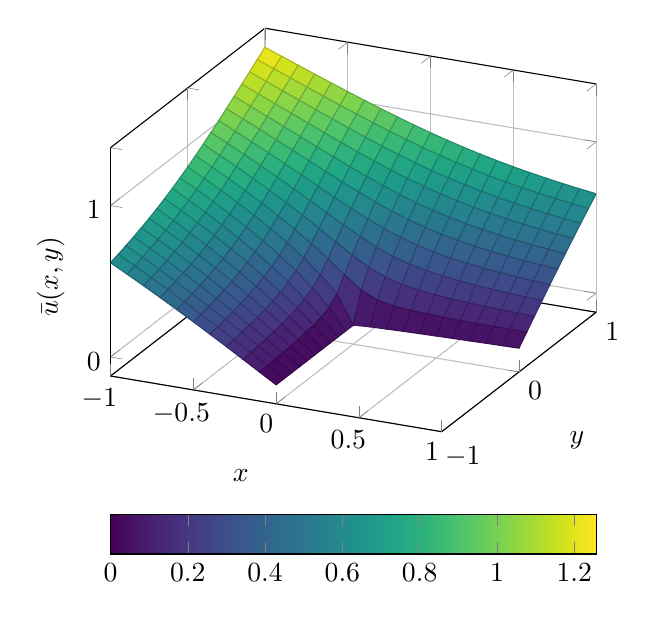
\begin{tikzpicture}
    \begin{axis}[
    scale=0.9,
    grid=major,
    colorbar horizontal,
    colormap/viridis,
    xlabel=$x$,
    ylabel=$y$,
    zlabel={$\bar{u}(x,y)$}
    ]
    \addplot3[
    surf,
    domain=-1:1,
    y domain=-1:1,
    restrict expr to domain={(x>0)&&(y<0)}{0:0},
    samples=21
    ]{pow(x*x+y*y,0.33)*sin(0.66*(atan2(y,-x)+90)))};
    \end{axis}
    \end{tikzpicture}
  }
  \caption{L-shaped domain}
  \end{figure}
\end{minipage}
\end{frame}





\begin{frame}
\frametitle{Example: Successive refinement}

\begin{itemize}
\item Initialize coarse mesh
\item Solve and refine in multiple cycles for tailored discretization
\end{itemize}

\begin{figure}
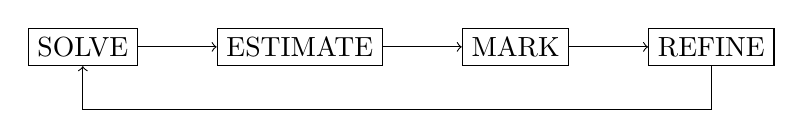
\begin{tikzpicture}[block/.style={draw}]%, node distance=.35cm]
\node [block] (solve) {SOLVE};
\node [block, right=of solve] (estimate) {ESTIMATE};
\node [block, right=of estimate] (mark) {MARK};
\node [block, right=of mark] (refine) {REFINE};

\draw[->] (solve) -- (estimate);
\draw[->] (estimate) -- (mark);
\draw[->] (mark) -- (refine);
\draw[->] (refine) -- ($ (refine) + (0,-0.8) $)  -| (solve);
\end{tikzpicture}
\caption{Successive refinement}
\end{figure}

\begin{enumerate}
\item Calculate refinement criteria (here: error estimates)
\item Flag 30\%/3\% of cells with highest/lowest criterion for refinement/coarsening
\item Calculate decision criteria (here: smoothness estimates)
\item Flag 90\%/10\% for $p$-/$h$-adaptation
\end{enumerate}
\end{frame}





\begin{frame}
\frametitle{Example: Successive refinement}

\begin{figure}
\only<1>{
  \begin{tikzpicture}
  \begin{axis}[
  scale=1,
  xmin=-1,xmax=1,
  ymin=-1,ymax=1,
  unit vector ratio={1 1},
  tick align=outside,
  xlabel=$x$,
  ylabel=$y$,
  colormap/OrRd,
  colorbar sampled,
  colorbar style={ylabel={finite element polynomial degree}, samples=7, ytick={2,3,...,7}},
  colormap access=piecewise const,
  point meta min=1.5,
  point meta max=7.5
  ]
  
  \addplot graphics [
  xmin=-1,xmax=1,
  ymin=-1,ymax=1,
  ] {illustrations/corner-fedegrees-legendre-00.pdf};
  \end{axis}
  \end{tikzpicture}
  
  \caption{Polynomial degrees in cycle 0. Zoom 100\%.}
}
\only<2>{
  \begin{tikzpicture}
  \begin{axis}[
  scale=1,
  xmin=-1,xmax=1,
  ymin=-1,ymax=1,
  unit vector ratio={1 1},
  tick align=outside,
  xlabel=$x$,
  ylabel=$y$,
  colormap/OrRd,
  colorbar sampled,
  colorbar style={ylabel={finite element polynomial degree}, samples=7, ytick={2,3,...,7}},
  colormap access=piecewise const,
  point meta min=1.5,
  point meta max=7.5
  ]
  
  \addplot graphics [
  xmin=-1,xmax=1,
  ymin=-1,ymax=1,
  ] {illustrations/corner-fedegrees-legendre-01.pdf};
  \end{axis}
  \end{tikzpicture}
  
  \caption{Polynomial degrees in cycle 1. Zoom 100\%.}
}
\only<3>{
  \begin{tikzpicture}
  \begin{axis}[
  scale=1,
  xmin=-1,xmax=1,
  ymin=-1,ymax=1,
  unit vector ratio={1 1},
  tick align=outside,
  xlabel=$x$,
  ylabel=$y$,
  colormap/OrRd,
  colorbar sampled,
  colorbar style={ylabel={finite element polynomial degree}, samples=7, ytick={2,3,...,7}},
  colormap access=piecewise const,
  point meta min=1.5,
  point meta max=7.5
  ]
  
  \addplot graphics [
  xmin=-1,xmax=1,
  ymin=-1,ymax=1,
  ] {illustrations/corner-fedegrees-legendre-02.pdf};
  \end{axis}
  \end{tikzpicture}
  
  \caption{Polynomial degrees in cycle 2. Zoom 100\%.}
}
\only<4>{
  \begin{tikzpicture}
  \begin{axis}[
  scale=1,
  xmin=-1,xmax=1,
  ymin=-1,ymax=1,
  unit vector ratio={1 1},
  tick align=outside,
  xlabel=$x$,
  ylabel=$y$,
  colormap/OrRd,
  colorbar sampled,
  colorbar style={ylabel={finite element polynomial degree}, samples=7, ytick={2,3,...,7}},
  colormap access=piecewise const,
  point meta min=1.5,
  point meta max=7.5
  ]
  
  \addplot graphics [
  xmin=-1,xmax=1,
  ymin=-1,ymax=1,
  ] {illustrations/corner-fedegrees-legendre-03.pdf};
  \end{axis}
  \end{tikzpicture}
  
  \caption{Polynomial degrees in cycle 3. Zoom 100\%.}
}
\only<5>{
  \begin{tikzpicture}
  \begin{axis}[
  scale=1,
  xmin=-1,xmax=1,
  ymin=-1,ymax=1,
  unit vector ratio={1 1},
  tick align=outside,
  xlabel=$x$,
  ylabel=$y$,
  colormap/OrRd,
  colorbar sampled,
  colorbar style={ylabel={finite element polynomial degree}, samples=7, ytick={2,3,...,7}},
  colormap access=piecewise const,
  point meta min=1.5,
  point meta max=7.5
  ]
  
  \addplot graphics [
  xmin=-1,xmax=1,
  ymin=-1,ymax=1,
  ] {illustrations/corner-fedegrees-legendre-04.pdf};
  \end{axis}
  \end{tikzpicture}
  
  \caption{Polynomial degrees in cycle 4. Zoom 100\%.}
}
\only<6>{
  \begin{tikzpicture}
  \begin{axis}[
  scale=1,
  xmin=-1,xmax=1,
  ymin=-1,ymax=1,
  unit vector ratio={1 1},
  tick align=outside,
  xlabel=$x$,
  ylabel=$y$,
  colormap/OrRd,
  colorbar sampled,
  colorbar style={ylabel={finite element polynomial degree}, samples=7, ytick={2,3,...,7}},
  colormap access=piecewise const,
  point meta min=1.5,
  point meta max=7.5
  ]
  
  \addplot graphics [
  xmin=-1,xmax=1,
  ymin=-1,ymax=1,
  ] {illustrations/corner-fedegrees-legendre-05.pdf};
  \end{axis}
  \end{tikzpicture}
  
  \caption{Polynomial degrees in cycle 5. Zoom 100\%.}
}
\only<7>{
  \begin{tikzpicture}
  \begin{axis}[
  scale=1,
  xmin=-0.5,xmax=0.5,
  ymin=-0.5,ymax=0.5,
  unit vector ratio={1 1},
  tick align=outside,
  xlabel=$x$,
  ylabel=$y$,
  colormap/OrRd,
  colorbar sampled,
  colorbar style={ylabel={finite element polynomial degree}, samples=7, ytick={2,3,...,7}},
  colormap access=piecewise const,
  point meta min=1.5,
  point meta max=7.5
  ]
  
  \addplot graphics [
  xmin=-1,xmax=1,
  ymin=-1,ymax=1,
  ] {illustrations/corner-fedegrees-legendre-05.pdf};
  \end{axis}
  \end{tikzpicture}
  
  \caption{Polynomial degrees in cycle 5. Zoom 200\%.}
}
\only<8>{
  \begin{tikzpicture}
  \begin{axis}[
  scale=1,
  xmin=-0.25,xmax=0.25,
  ymin=-0.25,ymax=0.25,
  unit vector ratio={1 1},
  tick align=outside,
  xlabel=$x$,
  ylabel=$y$,
  colormap/OrRd,
  colorbar sampled,
  colorbar style={ylabel={finite element polynomial degree}, samples=7, ytick={2,3,...,7}},
  colormap access=piecewise const,
  point meta min=1.5,
  point meta max=7.5
  ]
  
  \addplot graphics [
  xmin=-1,xmax=1,
  ymin=-1,ymax=1,
  ] {illustrations/corner-fedegrees-legendre-05.pdf};
  \end{axis}
  \end{tikzpicture}
  
  \caption{Polynomial degrees in cycle 5. Zoom 400\%.}
}
\only<9>{
  \begin{tikzpicture}
  \begin{axis}[
  scale=1,
  xmin=-0.125,xmax=0.125,
  ymin=-0.125,ymax=0.125,
  scaled x ticks = false,
  x tick label style={/pgf/number format/fixed},
  scaled y ticks = false,
  y tick label style={/pgf/number format/fixed},
  unit vector ratio={1 1},
  tick align=outside,
  xlabel=$x$,
  ylabel=$y$,
  colormap/OrRd,
  colorbar sampled,
  colorbar style={ylabel={finite element polynomial degree}, samples=7, ytick={2,3,...,7}},
  colormap access=piecewise const,
  point meta min=1.5,
  point meta max=7.5
  ]
  
  \addplot graphics [
  xmin=-1,xmax=1,
  ymin=-1,ymax=1,
  ] {illustrations/corner-fedegrees-legendre-05.pdf};
  \end{axis}
  \end{tikzpicture}
  
  \caption{Polynomial degrees in cycle 5. Zoom 800\%.}
}
\end{figure}
\end{frame}





\begin{frame}
\frametitle{Example: Successive refinement}

\begin{minipage}{1.08\textwidth}
  \begin{figure}
    \hspace{-1cm}
    \begin{subfigure}{.32\textwidth}
    \centering
    \begin{tikzpicture}
    \begin{axis}[
    scale=0.72,
    xmin=-1,xmax=1,
    ymin=-1,ymax=1,
    ticks=none,
    unit vector ratio={1 1},
    ]
    
    \addplot graphics [
    xmin=-1,xmax=1,
    ymin=-1,ymax=1,
    ] {illustrations/corner-fedegrees-fourier-05.pdf};
    \end{axis}
    \end{tikzpicture}
    \caption{Fourier coefficient decay}
    \end{subfigure}
    \begin{subfigure}{.32\textwidth}
    \centering
    \begin{tikzpicture}
    \begin{axis}[
    scale=0.72,
    xmin=-1,xmax=1,
    ymin=-1,ymax=1,
    ticks=none,
    unit vector ratio={1 1},
    ]
    
    \addplot graphics [
    xmin=-1,xmax=1,
    ymin=-1,ymax=1,
    ] {illustrations/corner-fedegrees-legendre-05.pdf};
    \end{axis}
    \end{tikzpicture}
    \caption{Legendre coefficient decay}
    \end{subfigure}
    \begin{subfigure}{.32\textwidth}
    \centering
    \begin{tikzpicture}
    \begin{axis}[
    scale=0.72,
    xmin=-1,xmax=1,
    ymin=-1,ymax=1,
    ticks=none,
    unit vector ratio={1 1},
    ]
    
    \addplot graphics [
    xmin=-1,xmax=1,
    ymin=-1,ymax=1,
    ] {illustrations/corner-fedegrees-prediction-05.pdf};
    \end{axis}
    \end{tikzpicture}
    \caption{Refinement history}
  \end{subfigure}
  \caption{Mesh and polynomial degrees of finite elements after 5 consecutive \newline $hp$-adaptations.}
  \end{figure}
\end{minipage}
\end{frame}




\begin{frame}
\frametitle{Example: Successive refinement}

\begin{figure}
\begin{tikzpicture}
\begin{loglogaxis}[
scale=1,
xlabel={Number of degrees of freedom},
ylabel={H1 error},
grid=major,
legend cell align=left,
legend pos=outer north east,
]
\addplot table [y=H1 error, x=ndofs, col sep=comma] {data/error/hp-legendre.csv};
\addlegendentry{\hp{} Legendre};

\addplot table [y=H1 error, x=ndofs, col sep=comma] {data/error/hp-fourier.csv};
\addlegendentry{\hp{} Fourier};

\addplot table [y=H1 error, x=ndofs, col sep=comma] {data/error/hp-prediction.csv};
\addlegendentry{\hp{} prediction};

\addplot table [y=H1 error, x=ndofs, col sep=comma] {data/error/h.csv};
\addlegendentry{\h};
\end{loglogaxis}
\end{tikzpicture}
\caption{Error convergence for different strategies}
\end{figure}
\end{frame}
\section{Parallelization}





\begin{frame}
\frametitle{Table of contents}

\tableofcontents[currentsection]
\end{frame}





\begin{frame}
\frametitle{Parallelization}

\begin{itemize}
\item Current computer architectures provide multi-core processors
  \begin{itemize}
  \item Supercomputers arrange those on distributed nodes
  \end{itemize}
\item Using all resources efficiently requires parallelization
  \begin{itemize}
  \item Distribution of workload and memory demand
  \end{itemize}
\end{itemize}

\begin{itemize}
\item Our approach: Distribution of domain on several processes
  \begin{itemize}
  \item Each subdomain needs relevant part of the global solution
  \item Requires a layer of so called ghost cells
  \item Involves communication between processors
  \end{itemize}
\end{itemize}

\begin{figure}
\begin{subfigure}{.31\textwidth}
  \centering
  \begin{tikzpicture}
  \LagrangeCell{0}{0}{1}{.08}{1}
  {{"","","",""}};
  \LagrangeCell{1}{0}{1}{.08}{1}
  {{"","","",""}};
  \LagrangeCell{2}{0}{1}{.08}{1}
  {{"","","",""}};
  \end{tikzpicture}
  \caption{Domain to be distributed}
\end{subfigure}
\hspace{-.9ex}\raisebox{.5em}{\(\longrightarrow\)}
\begin{subfigure}{.3\textwidth}
  \centering
  \begin{tikzpicture}
  \fill[color=fzjblue] (0,0) rectangle (1,1);
  \fill[color=fzjblue] (1,0) rectangle (2,1);
  \fill[color=fzjlightblue] (2,0) rectangle (3,1);
  
  \LagrangeCell{0}{0}{1}{.08}{1}
  {{"","","",""}};
  \LagrangeCell{1}{0}{1}{.08}{1}
  {{"","","",""}};
  \LagrangeCell{2}{0}{1}{.08}{1}
  {{"","","",""}};
  \end{tikzpicture}
  \caption{Subdomain for CPU 0}
\end{subfigure}
\begin{subfigure}{.3\textwidth}
  \centering
  \begin{tikzpicture}
  \fill[color=lightgray] (0,0) rectangle (1,1);
  \fill[color=fzjlightblue] (1,0) rectangle (2,1);
  \fill[color=fzjblue] (2,0) rectangle (3,1);
  
  \LagrangeCell{0}{0}{1}{.08}{1}
  {{"","","",""}};
  \LagrangeCell{1}{0}{1}{.08}{1}
  {{"","","",""}};
  \LagrangeCell{2}{0}{1}{.08}{1}
  {{"","","",""}};
  \end{tikzpicture}
  \caption{Subdomain for CPU 1}
\end{subfigure}
%  \vspace{-.3em}
\caption{Illustration of \textcolor{black!10!fzjblue}{\textbf{locally owned}}, \textcolor{black!10!fzjlightblue}{\textbf{ghost}}, and \textcolor{black!10!lightgray}{\textbf{artificial}} cells}
\end{figure}
\end{frame}





\begin{frame}
\frametitle{Parallel hp-adaptive FEM}

\begin{itemize}
\item Combination of hp-adaptive methods with parallelisation
\end{itemize}

\vfill{}

\begin{itemize}
\item The non-trivial parts are:
  \begin{enumerate}
  \item Enumeration of degrees of freedom, independent of number of subdomains
  \item Consignment of contiguous memory chunks for data transfer
  \item Weighted repartitioning for load balancing
  \end{enumerate}
\end{itemize}

\vfill{}

\begin{figure}
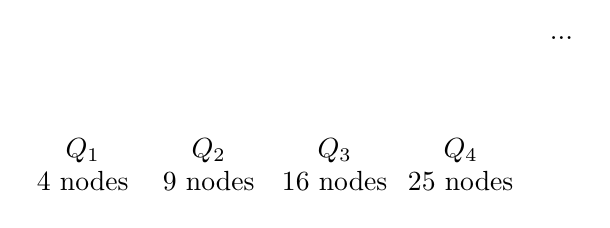
\begin{tikzpicture}[scale=1.6]
\node[align=center] at ( .5,-.5) {$Q_1$ \\  4 nodes};
\node[align=center] at (1.5,-.5) {$Q_2$ \\  9 nodes};
\node[align=center] at (2.5,-.5) {$Q_3$ \\ 16 nodes};
\node[align=center] at (3.5,-.5) {$Q_4$ \\ 25 nodes};

\LagrangeCell{0}{0}{1}{.04}{1}
{{,,,}};
\LagrangeCell{1}{0}{1}{.04}{2}
{{,,,,,,,,}};
\LagrangeCell{2}{0}{1}{.04}{3}
{{,,,,,,,,,,,,,,,}};
\LagrangeCell{3}{0}{1}{.04}{4}
{{,,,,,,,,,,,,,,,,,,,,,,,,,}};

\node at (4.3,.5) {...};
\end{tikzpicture}
\caption{Different finite elements and their number of nodes in 2D}
\end{figure}
\end{frame}





\subsection{Example: Laplace equation}





\begin{frame}
\frametitle{Example: Load balancing}

\begin{figure}
\only<1>{
  \vspace{-.7em}
  \begin{tikzpicture}
  \begin{axis}[
  scale=1,
  xmin=-1,xmax=1,
  ymin=-1,ymax=1,
  unit vector ratio={1 1},
  tick align=outside,
  xlabel=$x$,
  ylabel=$y$,
  colormap/Paired,
  colorbar sampled,
  colorbar style={ylabel={subdomain}, samples=13, ytick={0,1,...,11}},
  colormap access=piecewise const,
  point meta min=-.5,
  point meta max=11.5
  ]
  
  \addplot graphics [
  xmin=-1,xmax=1,
  ymin=-1,ymax=1,
  ] {figures/corner-subdomains-legendre-00.pdf};
  \end{axis}
  \end{tikzpicture}
  \vspace{-.7em}
  \caption{Mesh decomposition in cycle 0.
Weights assigned to cells are $\propto n_\text{dofs}^{1.9}$.}
}
\only<2>{
  \vspace{-.7em}
  \begin{tikzpicture}
  \begin{axis}[
  scale=1,
  xmin=-1,xmax=1,
  ymin=-1,ymax=1,
  unit vector ratio={1 1},
  tick align=outside,
  xlabel=$x$,
  ylabel=$y$,
  colormap/Paired,
  colorbar sampled,
  colorbar style={ylabel={subdomain}, samples=13, ytick={0,1,...,11}},
  colormap access=piecewise const,
  point meta min=-.5,
  point meta max=11.5
  ]
  
  \addplot graphics [
  xmin=-1,xmax=1,
  ymin=-1,ymax=1,
  ] {figures/corner-subdomains-legendre-01.pdf};
  \end{axis}
  \end{tikzpicture}
  \vspace{-.7em}
  \caption{Mesh decomposition in cycle 1.
Weights assigned to cells are $\propto n_\text{dofs}^{1.9}$.}
}
\only<3>{
  \vspace{-.7em}
  \begin{tikzpicture}
  \begin{axis}[
  scale=1,
  xmin=-1,xmax=1,
  ymin=-1,ymax=1,
  unit vector ratio={1 1},
  tick align=outside,
  xlabel=$x$,
  ylabel=$y$,
  colormap/Paired,
  colorbar sampled,
  colorbar style={ylabel={subdomain}, samples=13, ytick={0,1,...,11}},
  colormap access=piecewise const,
  point meta min=-.5,
  point meta max=11.5
  ]
  
  \addplot graphics [
  xmin=-1,xmax=1,
  ymin=-1,ymax=1,
  ] {figures/corner-subdomains-legendre-02.pdf};
  \end{axis}
  \end{tikzpicture}
  \vspace{-.7em}
  \caption{Mesh decomposition in cycle 2.
Weights assigned to cells are $\propto n_\text{dofs}^{1.9}$.}
}
\only<4>{
  \vspace{-.7em}
  \begin{tikzpicture}
  \begin{axis}[
  scale=1,
  xmin=-1,xmax=1,
  ymin=-1,ymax=1,
  unit vector ratio={1 1},
  tick align=outside,
  xlabel=$x$,
  ylabel=$y$,
  colormap/Paired,
  colorbar sampled,
  colorbar style={ylabel={subdomain}, samples=13, ytick={0,1,...,11}},
  colormap access=piecewise const,
  point meta min=-.5,
  point meta max=11.5
  ]
  
  \addplot graphics [
  xmin=-1,xmax=1,
  ymin=-1,ymax=1,
  ] {figures/corner-subdomains-legendre-03.pdf};
  \end{axis}
  \end{tikzpicture}
  \vspace{-.7em}
  \caption{Mesh decomposition in cycle 3.
Weights assigned to cells are $\propto n_\text{dofs}^{1.9}$.}
}
\only<5>{
  \vspace{-.7em}
  \begin{tikzpicture}
  \begin{axis}[
  scale=1,
  xmin=-1,xmax=1,
  ymin=-1,ymax=1,
  unit vector ratio={1 1},
  tick align=outside,
  xlabel=$x$,
  ylabel=$y$,
  colormap/Paired,
  colorbar sampled,
  colorbar style={ylabel={subdomain}, samples=13, ytick={0,1,...,11}},
  colormap access=piecewise const,
  point meta min=-.5,
  point meta max=11.5
  ]
  
  \addplot graphics [
  xmin=-1,xmax=1,
  ymin=-1,ymax=1,
  ] {figures/corner-subdomains-legendre-04.pdf};
  \end{axis}
  \end{tikzpicture}
  \vspace{-.7em}
  \caption{Mesh decomposition in cycle 4.
Weights assigned to cells are $\propto n_\text{dofs}^{1.9}$.}
}
\only<6>{
  \vspace{-.7em}
  \begin{tikzpicture}
  \begin{axis}[
  scale=1,
  xmin=-1,xmax=1,
  ymin=-1,ymax=1,
  unit vector ratio={1 1},
  tick align=outside,
  xlabel=$x$,
  ylabel=$y$,
  colormap/Paired,
  colorbar sampled,
  colorbar style={ylabel={subdomain}, samples=13, ytick={0,1,...,11}},
  colormap access=piecewise const,
  point meta min=-.5,
  point meta max=11.5
  ]
  
  \addplot graphics [
  xmin=-1,xmax=1,
  ymin=-1,ymax=1,
  ] {figures/corner-subdomains-legendre-05.pdf};
  \end{axis}
  \end{tikzpicture}
  \vspace{-.7em}
  \caption{Mesh decomposition in cycle 5.
Weights assigned to cells are $\propto n_\text{dofs}^{1.9}$.}
}
\end{figure}
\end{frame}




\begin{frame}
\frametitle{Example: Strong scaling}

\vspace{-1em}

\begin{figure}
\begin{tikzpicture}
\begin{loglogaxis}[
scale=0.9,
xlabel={Number of MPI processes},
ylabel={Wall time [seconds]},
grid=major,
legend cell align=left,
legend pos=outer north east,
legend style={font=\tiny}
]
% data
\addplot table [y=solve, x=ncpus, col sep=comma] {data/strong/strong-nrefs12.csv};
\addlegendentry{linear solver and preconditioner};

\addplot table [y=setup, x=ncpus, col sep=comma] {data/strong/strong-nrefs12.csv};
\addlegendentry{setup data structures};

\addplot table [y=assembly, x=ncpus, col sep=comma] {data/strong/strong-nrefs12.csv};
\addlegendentry{assemble linear system};

\addplot table [y=compute errors, x=ncpus, col sep=comma] {data/strong/strong-nrefs12.csv};
\addlegendentry{estimate error};

\addplot table [y=calculate indicators, x=ncpus, col sep=comma] {data/strong/strong-nrefs12.csv};
\addlegendentry{estimate smoothness};

\addplot table [y=refine, x=ncpus, col sep=comma] {data/strong/strong-nrefs12.csv};
\addlegendentry{coarsen and refine};

% optimal line
\addplot[very thick, samples=2, domain=768:49152] {10^(5)*x^(-1)};
\addlegendentry{optimal convergence};

% auxiliary lines
\begin{scope}
\draw[green, very thick] ({axis cs:9692.57276,0}|-{rel axis cs:0,1}) -- ({axis cs:9692.57276,0}|-{rel axis cs:0,0});
\end{scope}
\addlegendimage{color=green};
\addlegendentry{$10^5$ DoFs per process};
\end{loglogaxis}
\end{tikzpicture}
\caption{Strong scaling for fixed problem size of $\sim$ 970 million degrees of freedom}
\end{figure}
\end{frame}
\chapter{Summary and outlook}
\label{ch:summary}
\glsresetall

% summary

The \gls{fem} offers the unique capability of \hp-adaptive methods with remarkable properties in error convergence relative to workload. However for \gls{hpc}, their parallel implementation for large scale computing architectures with distributed memory via \gls{mpi} is difficult.

We presented generic algorithms and data structures for massively parallel \hp-adaptive \gls{fem}, which allow for dynamic changes in both grid resolution and assignment of finite elements. Our findings are independent of the implementation and can be used to enhance any kind of \gls{fem} software, provided that their concepts conform to the elementary work of \textcite{bangerth2009,bangerth2012}, which forms the basis of our research.

%can be enhanced with these findings, provided they already feature parallel \h-adaptive and sequential \hp-adaptive methods by \textcite{bangerth2009,bangerth2012}.

%provided that their underlying structure is compatible with 

%which can be used to enhance any existing \gls{fem} software. 

In this dissertation, we elaborated on the non-trivial parts of combining both parallel \h-adaptive and sequential \hp-adaptive methods.
%, which are briefly recapped in the following:
%\begin{itemize}
%\item%
The unique enumeration of \glspl{dof} and their affiliation with the owning \gls{mpi} process poses challenges for \gls{cg} methods whenever finite elements of similar or different polynomial degree meet on subdomain boundaries. We developed an algorithm for the unique enumeration of \glspl{dof} in the parallel \hp-adaptive context which does not require more costly communication with ghost cells than the \h-adaptive pendant.

%\item%
For an automatic adaptation, refinement criteria on basis of error indicators are required to decide which parts of the domain should be adapted. In addition using \hp-adaptive methods, we also have to select the type of adaptation we would like to impose.
%In addition to the determination of refinement criteria on basis of error indicators, we need to additionally decide which type of adaptation to impose for an automatic determination.
We presented several state-of-the-art methods for \hp-refinement, prepared them for parallel applications, and enhanced them for \hp-coarsening as well.
%\end{itemize}

%\item%
Cells are distributed on \gls{mpi} processes in such a way that the workload is balanced among them, which we ensure by a weighted repartitioning. On each cell, we imposed a simple weight proportional to the \glspl{dof} potentiated by a factor which depends on the problem to investigate.

%\item%
Whenever the mesh itself changes in parallel applications, for example by adaptation, workload needs to be redistributed by repartitioning. Depending on the investigated problem, transferring data from the former to the updated mesh is necessary, for example the finite element approximation itself. In addition using \hp-adaptive methods, the amount of data to be transferred might vary by cell. We present a general approach to provide contiguous memory sections which will be exchanged using optimized algorithms presented by \textcite{burstedde2018} for data of fixed and variable size, respectively.

%We use optimized algorithms presented by .

%Data transfer of variable size via \gls{mpi} and the necessity of contiguous memory chunks to easily address each processor's locally owned space.

We provided a reference implementation in the \dealii{} library and applied it to the Laplace problem on an L-shaped domain, a common numerical benchmark for \hp-adaptive methods. We have demonstrated their superior error convergence and shown that our implementation scales on up to 49,152 \gls{mpi} processes.

%While sequential, static \hp-adaptive methods have been frequently used in multi-physics problems in \dealii{}, the actual application of dynamic \hp-adaptive methods stayed mostly in an experimental state within \dealii{} because of its intricate application. With the current interface as redesigned in this dissertation hopefully simplifies its usage so that it attracts for users and it hopefully becomes a widely used feature in the community.


% extensions

Algorithms for parallel \hp-adaptive \glspl{fem} capable of handling both \gls{cg} and \gls{dg} methods have not yet been prepared in a general framework like this before. However, our implementation is still at an early stage of development, and there is still plenty of room for improvement, as we described throughout this dissertation. Those aspects that leave room for improvements are the following.

We observed an unfavorable scaling behavior during the solution of the equation system in our \hp-adaptive \gls{fem} application, which we attribute to our choice of \gls{amg} preconditioning. A preconditioner that also incorporates multilevel methods on a hierarchy of finite elements with different polynomial degrees $p$ will be more efficient and solve the linear equation system in less iterations as investigated by \textcite{mitchell2010}. They embedded \p-multigrid methods in \gls{gmg} preconditioning for sequential \hp-adpative applications. Furthermore, \textcite{fehn2019} combined multilevel methods on hierarchies in a polynomial, geometric, and algebraic sense for parallel \gls{fem} on static meshes without adaptation. Future work involves the combination of multilevel methods to make them available for parallel \hp-adaptive methods as well.
This also incorporates parallel \h-adaptive \gls{gmg} preconditioners that have been presented by \textcite{clevenger2019} who also provided an implementation in the \dealii{} library.
%for which \gls{gmg} methods are promising. For parallel \h-adaptive \gls{fem}, \textcite{clevenger2019} presented algorithms for \gls{gmg} preconditioners and provided an implementation in the \dealii{} library. Future work involves enhancing them for \hp-adaptive methods as well, combining their ideas with those of \textcite{mitchell2010}.

%Geometric multigrid
%Find a way to combine the parallel \h-adpative \gls{gmg} preconditioner by \textcite{clevenger2019} with the \hp-adaptive variant by \textcite{mitchell2010}.

%how to combine them with the ideas of melenk for \hp-adaptive \gls{gmg} methods.

%new strategies to decide between \h- and \p-adaptation
We described a handful of decision strategies to choose between types of adaptation. However, there are more strategies worth trying out.
%Regularity estimation (see houston 2005 for references), houston 2003
%\textcite{houston2003} \textcite{houston2005}
\textcite{houston2003,houston2005} directly determined the regularity of the solution from the coefficients of a Legendre expansion of the finite element approximation. We could use those as decision indicators, or directly set the fitting finite element on basis of their result.
%Enhancements for Fourier strategy using \gls{fft} (e.g. via \fftw{} \parencite{frigo2005,fftw338}).
%Further, we noticed that the preparation of the Fourier transformation matrices consumes a lot of wall time due to the larger number of quadrature points required for integration, which we hope to accelerate using \gls{fft}, for example via \fftw{} \parencite{frigo2005,fftw338}.

One could also imagine different decision indicators that are specific to the investigated problem. Hence for computational fluid dynamics, we could relate the decision criteria towards a measure for turbulence for example. The absolute value of the vorticity $\vec{w} = (\nabla \times \vec{v})$ as the rotation of the fluid velocity $\vec{v}$ would make up a good measure. We would prefer \h-refinement on turbulent regions indicated by a high vorticity, and \p-refinement in laminar regions.

%Let us consider for examples computational fluid dynamics. We could use different criteria to decide for \hp-adaptation. The vorticity $\vec{w} = (\nabla \times \vec{v})$ or the dimensionless Reynolds number $\mathrm{Re} = (v L / \nu)$ would make up a good measure, with the velocity $\vec{v}$, the kinematic viscosity $\nu$ and a characteristic length $L$. We would prefer \h-refinement on turbulent regions indicated by a high vorticity or Reynolds number, and \p-refinement in laminar regions.

Future work will involve examining the possibility to combine \hp-adaptive methods with so called matrix-free methods. Memory access is the current bottleneck on \gls{hpc} machines. Instead of calculating matrix entries and storing them, it might be faster to calculate them on the fly as they are requested. Combined with \gls{simd} instructions or \gls{gpu} acceleration, this is a highly favorable strategy on current \gls{hpc} machines. Matrix-free methods have been part of the \dealii{} for a long time \parencite{kronbichler2012}, and have been continuously enhanced during the last decade \parencite{kronbichler2019}. Furthermore, \textcite{munch2020} recently published an open-source library named \texttt{hyper.deal} using high-order \gls{dg} methods for high-dimensional partial differential equations, which is built on top of \dealii{} and provides an easy-to-use interface to utilize these methods. The purpose of their framework is to investigate the dynamics of plasmas in nuclear fusion reactors involving shocks, which are modeled using the six-dimensional Vlasov equation. An extension with \hp-adaptive methods would be highly promising in any case and would unleash their full potential. A specialized decision strategy for \hp-adaptation tied to an observable might be more suitable in the context of plasmas than the general strategies presented in this project.

More generally, this framework can also be used to solve many other problems in continuum mechanics as well, e.g., structural mechanics and fluid dynamics in general. As a concrete application example in geosciences, convection processes in Earth's mantle can be simulated with the open-source code \texttt{ASPECT} \parencite{kronbichler2012a,aspect210} which builds upon the \dealii{} library. Simulation on a domain of planetary scope yields a lot of workload. Thus \texttt{ASPECT} already benefits tremendously from parallel \h-adaptive methods, and now also has parallel \hp-adaptive methods at its disposal with the results of our project.


% closing words

We are left to see whether \hp-adaptive \gls{fem} for architectures with distributed memory will be well-received by the community. At the very least, it has been a long requested feature of the \dealii{} library, which was first mentioned in the \dealii{} Google group\footnote{\url{https://groups.google.com/d/msg/dealii/BmEF75lOA_E/PjyF9F5Uo3UJ}} in early 2014 and has been in progress since late 2016 \textcite{dealiiissue3511}.

In the past, \textcite{bangerth2009} provided algorithms and data structures for sequential \hp-adaptive methods and provided a reference implementation in \dealii{}. They have been widely used for multi-physics problems in \dealii{}, coupling different physical models in different parts of the domain by assigning corresponding finite elements. However, automatic \hp-adaptation stayed mostly in an experimental state within \dealii{} because of its intricate application. The current interface has been redesigned in this project and simplifies its usage, so that it hopefully becomes a widely used feature in the community.

A good approach to make these features more accessible to all users of the library is to write a dedicated tutorial program as part of the \dealii{} library that showcases the new functionality presented in this dissertation. Tutorial programs are meant to demonstrate certain features of the library and give newcomers a fundamental insight into the numerical and computational background, as well as into implementation details due to extensive documentation.
%The \dealii{} library currently features a total of 62 of such tutorial programs in their most recent release \parencite{arndt2019}.
For the demonstration of parallel \hp-adaptive \gls{fem}, we will translate the numerical example from Ch.~\ref{ch:results} into a new stand-alone tutorial as a next step.

% We are left to provide an easily accessible tutorial program describing all features in the tradition of the \dealii{} library.

%Time will tell how this feature is going to be perceived by the scientific community.

%It has been a long requested feature in the \dealii{} library, which was first mentioned in the \dealii{} Google group\footnote{\url{https://groups.google.com/forum/\#!forum/dealii}} in late 2015, and work began in late 2016 \textcite{dealiiissue3511}.

% has now finally been implemented in a way that it is easily accessible by made

%It was first requested by the community as a feature mentioned in late 2015 in the deal.
%The first mention in the \dealii{} Google group\footnote{\url{https://groups.google.com/forum/\#!forum/dealii}} happened in late 2015, and work began in late 2016 \textcite{dealiiissue3511}.

After all, parallel \hp-adaptive methods offer promising capabilities, and with all features left to add they are a very challenging yet exciting topic worth to continue working on.

%And if the scientific interest will be underwhelming, we can at least still create nice pictures with it.

\appendix
\title{Massively parallel hp-adaptive FEM}
\subtitle{Bibliography}
\maketitle
\begin{frame}[allowframebreaks]
\frametitle{Bibliography}
\nocite{ainsworth1998,arndt2019,burstedde2018,eibner2007,houston2005,mitchell2014}
\setlength{\labelwidth}{\labelnumberwidth}
\printbibliography[title=Bibliography]
\end{frame}

\subtitle{Expected questions}
\maketitle
\begin{frame}
\frametitle{INS assumptions}

\begin{itemize}
  \item Incompressibility assumption: Mach number $< 0.3$
  \item Buoyancy force with Boussinesq approximation: $f \approx \rho_0 g - \rho_0 g \beta (T-T_0)$
\end{itemize}
\end{frame}





\begin{frame}
\frametitle{Karniadakis scheme}

\begin{itemize}
  \item Explicit convection step
  
    $(u^* - u^n)/k = - \nabla \cdot (u^nu^n) + f^{n+1}$
  \item Pressure Poisson equation and velocity reconstruction
  
    $\nabla^2 p^{n+1} = - 1/k \, \nabla \cdot u^*$
    
    $u^{**} = u^* - k \, \nabla p^{n+1}$
  \item Implicit diffusion step
  
    $ (u^{n+1} - u^{**})/k = \nabla \cdot (2\nu\epsilon) $
\end{itemize}
\end{frame}
\begin{frame}
\frametitle{Dimensionless quantities}

\begin{itemize}
\item Reynolds number: inertial/viscous forces (turbulence behavior)
\item Rayleigh number: time scales for thermal transport diffusion/convection
\item Grashof number: buoyant/viscous forces
\item Prandtl number: momentum/thermal diffusivity
\end{itemize}
\end{frame}
\begin{frame}
\frametitle{Types of PDEs}

General form of second order PDE with two variables
\begin{align*}
Au_{xx} + 2 Bu_{xy} + Cu_{yy} + Du_{x} + Eu_{y} + + Fu + G = 0
\end{align*}


\begin{itemize}
\item Elliptic equations: $B^2 - AC < 0$

  Laplace equation: $- u_{xx} - u_{yy} = 0$
\item Hyperbolic equations: $B^2 - AC > 0$

  Wave equation: $u_{tt} - c^2 u_{xx} = 0$
\item Parabolic equations: $B^2 - AC = 0$

  Heat equation: $u_{t} - \alpha u_{xx} = 0$
\end{itemize}
\end{frame}
\begin{frame}
\frametitle{Artificial cells}

\begin{itemize}
\item Every process knows about global coarse mesh
\item Correct level representation only on locally owned cells
\item 2:1 mesh balance
\item Artificial cells as coarse as possible
\end{itemize}

\vfill{}

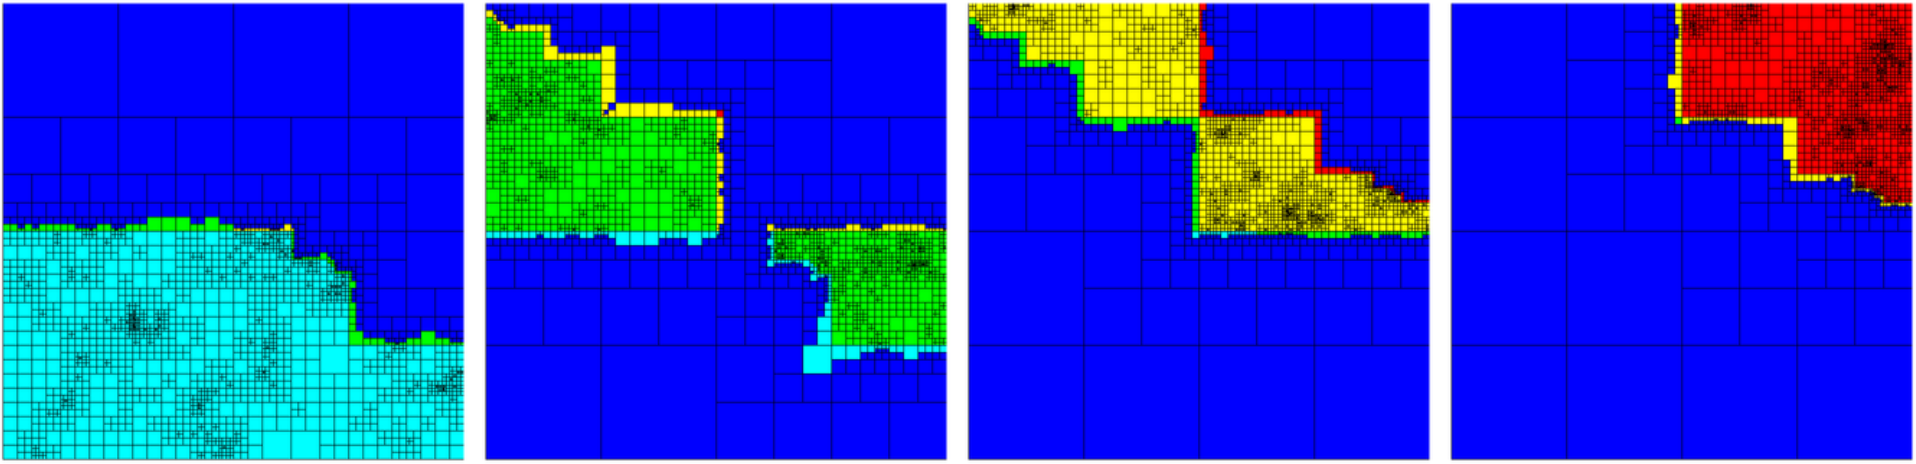
\includegraphics[width=\textwidth]{addendum/figures/artificial.png}
\end{frame}
\begin{frame}
\frametitle{Space-filling curve}

\begin{itemize}
\item Z-order space filling curve
\item Partitioning via leaves of tree structure
\end{itemize}

\vfill{}

\begin{figure}
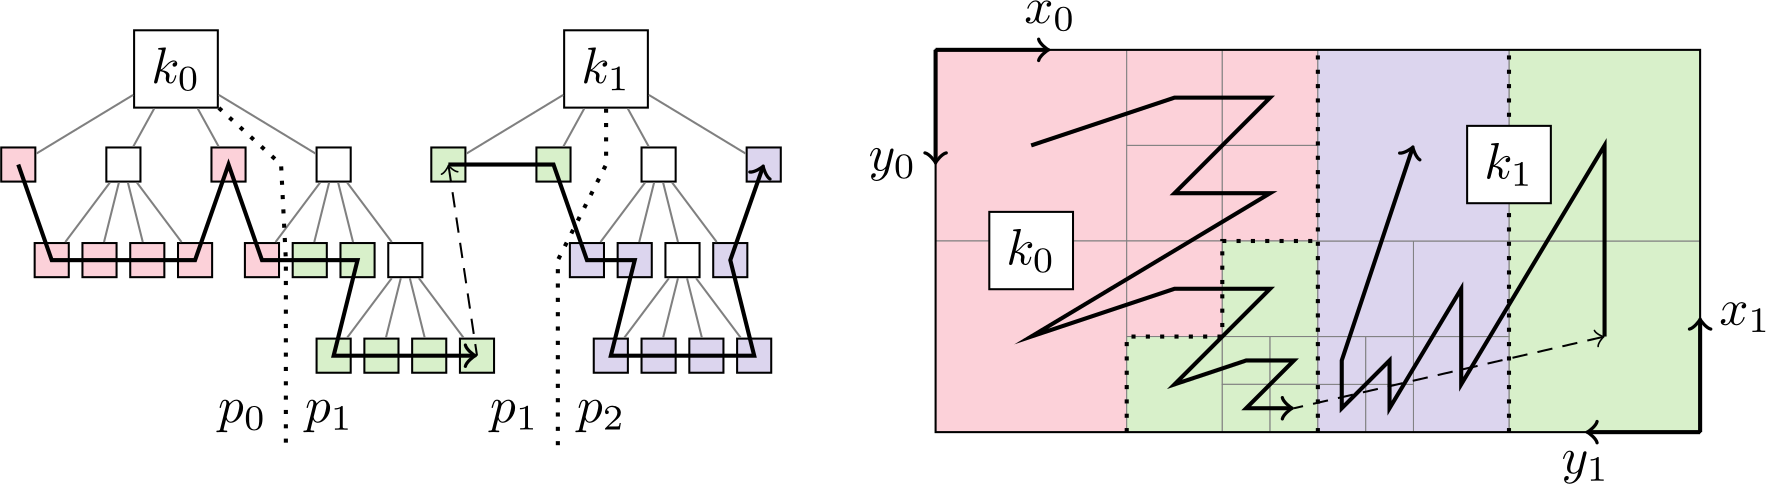
\includegraphics[width=\textwidth]{addendum/figures/p4est-forest-domain.png}
\caption{Correspondence of hierarchic tree structure and geometry, incorporating partitioning and the space-filling curve}
\end{figure}
\end{frame}

\subtitle{Details on algorithms}
\maketitle
\begin{frame}
\frametitle{Finite element method}

\begin{itemize}
\item Solve variational equation from 'weak' formulation of the differential equation with bilinear form \(a(u,v)\):
\begin{align*}
\exists u \in V: \forall v \in V: a(u,v) = f(v)
\end{align*}
\item Choose subspace \(V_\text{h}\) with basis \(w_\text{i}\), out of which the approximate solution \(u_\text{h} = \sum u_i w_i \in V_\text{h}\) will be constructed:
\begin{align*}
a(u_\text{h},w_\text{j}) = \sum\limits_i a(w_i,w_\text{j}) \; u_i = f(w_\text{j}) \quad\rightarrow\quad AU = F
\end{align*}
\end{itemize}

\vspace{-0.5em}

\begin{figure}
\hfill{}
\begin{subfigure}{0.2\textwidth}
  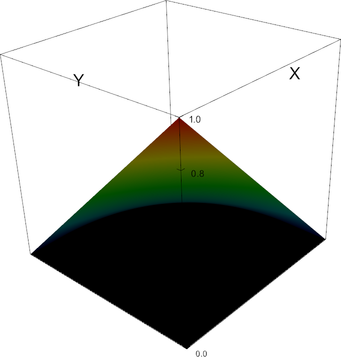
\includegraphics[width=\textwidth]{addendum/figures/Q1_shape0000.png}
\end{subfigure}
\hfill{}
\begin{subfigure}{0.2\textwidth}
  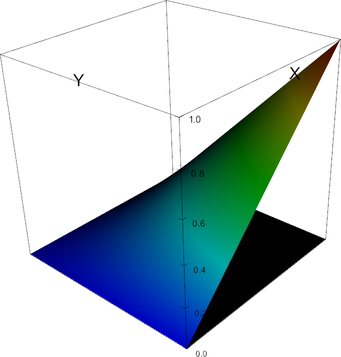
\includegraphics[width=\textwidth]{addendum/figures/Q1_shape0001.png}
\end{subfigure}
\hfill{}
\begin{subfigure}{0.2\textwidth}
  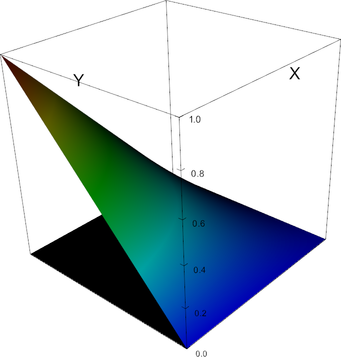
\includegraphics[width=\textwidth]{addendum/figures/Q1_shape0002.png}
\end{subfigure}
\hfill{}
\begin{subfigure}{0.2\textwidth}
  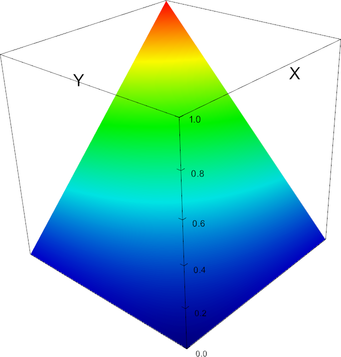
\includegraphics[width=\textwidth]{addendum/figures/Q1_shape0003.png}
\end{subfigure}
\hfill{}
\caption{\(Q_1\) elements in 2D
%  \tiny (source: \href{https://www.dealii.org/8.4.1/doxygen/deal.II/classFE__Q.html}{\underline{deal.II}}) \normalsize
}
\end{figure}
\end{frame}





\begin{frame}
\frametitle{Laplace equation}

Multiply with test function, integrate and apply Gauss theorem
\begin{align*}
- \nabla^2 u &= f \\
- \int_\Omega \nabla^2 u \varphi &= \int_\Omega \nabla u \nabla \varphi - \int_{\partial\Omega} \left(\vectorsym{n} \cdot \nabla\vectorsym{u}\right) \varphi = \int_\Omega f
\end{align*}

$\varphi = 0$ on boundary
\begin{align*}
(\nabla u, \nabla \varphi) &= (f,\varphi)
\end{align*}

Discretized
\begin{align*}
\sum_j \left(\nabla\varphi_i, \nabla \varphi_j \right) u_j &= (f,\varphi_i) \\
AU &= F
\end{align*}
\end{frame}





%\begin{frame}
%\frametitle{Mapping}
%  content...
%\end{frame}





\begin{frame}
\frametitle{Gaussian quadrature}
  
\begin{align*}
  A^K_{ij} &= \int_K \nabla\varphi_i \cdot \nabla \varphi_j \approx \sum_q \nabla\varphi_i(\mathbf x^K_q) \cdot \nabla \varphi_j(\mathbf x^K_q) w_q^K, \\
  F^K_i &= \int_K \varphi_i f \approx \sum_q \varphi_i(\mathbf x^K_q) f(\mathbf x^K_q) w^K_q,
\end{align*}
\end{frame}
\begin{frame}
\frametitle{Choose finite elements upon adaptation}

\begin{figure}
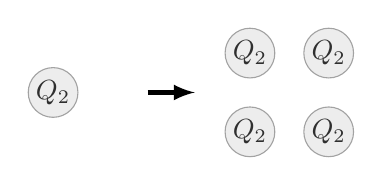
\begin{tikzpicture}[>=latex]
\def\Length{1}
\def\Radius{0.07}

% pre refinement
\LagrangeCell{0}{0}{2*\Length}{\Radius}{2}
{{,,,,,,,,}};
\node[circle, draw=gray, fill=gray!20, inner sep=1pt, opacity=0.7, text opacity=0.8] at (\Length,\Length) {$Q_2$};

% arrow
\draw[->,ultra thick] (2.2*\Length,\Length) -- (2.8*\Length,\Length);

% post refinement
\LagrangeCell{3*\Length}{0}{\Length}{\Radius}{2}
{{,,,,,,,,}};
\node[circle, draw=gray, fill=gray!20, inner sep=1pt, opacity=0.7, text opacity=0.8] at (3.5*\Length,0.5*\Length) {$Q_2$};

\LagrangeCell{4*\Length}{0}{\Length}{\Radius}{2}
{{,,,,,,,,}};
\node[circle, draw=gray, fill=gray!20, inner sep=1pt, opacity=0.7, text opacity=0.8] at (4.5*\Length,0.5*\Length) {$Q_2$};

\LagrangeCell{3*\Length}{\Length}{\Length}{\Radius}{2}
{{,,,,,,,,}};
\node[circle, draw=gray, fill=gray!20, inner sep=1pt, opacity=0.7, text opacity=0.8] at (3.5*\Length,1.5*\Length) {$Q_2$};

\LagrangeCell{4*\Length}{\Length}{\Length}{\Radius}{2}
{{,,,,,,,,}};
\node[circle, draw=gray, fill=gray!20, inner sep=1pt, opacity=0.7, text opacity=0.8] at (4.5*\Length,1.5*\Length) {$Q_2$};
\end{tikzpicture}
\caption{\hp{} refinement}
\end{figure}

\begin{figure}
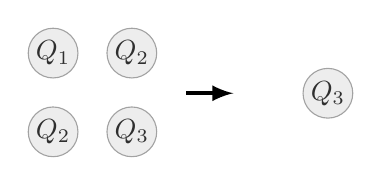
\begin{tikzpicture}[>=latex]
\def\Length{1}
\def\Radius{0.07}

% pre coarsening
\LagrangeCell{0}{0}{\Length}{\Radius}{2}
{{,,,,,,,,}};
\node[circle, draw=gray, fill=gray!20, inner sep=1pt, opacity=0.7, text opacity=0.8] at (0.5\Length,0.5\Length) {$Q_2$};

\LagrangeCell{\Length}{0}{\Length}{\Radius}{3}
{{,,,,,,,,,,,,,,,}};
\node[circle, draw=gray, fill=gray!20, inner sep=1pt, opacity=0.7, text opacity=0.8] at (1.5\Length,0.5\Length) {$Q_3$};

\LagrangeCell{0}{\Length}{\Length}{\Radius}{1}
{{,,,}};
\node[circle, draw=gray, fill=gray!20, inner sep=1pt, opacity=0.7, text opacity=0.8] at (0.5\Length,1.5\Length) {$Q_1$};

\LagrangeCell{\Length}{\Length}{\Length}{\Radius}{2}
{{,,,,,,,,}};
\node[circle, draw=gray, fill=gray!20, inner sep=1pt, opacity=0.7, text opacity=0.8] at (1.5\Length,1.5\Length) {$Q_2$};

% arrow
\draw[->,ultra thick] (2.2*\Length,\Length) -- (2.8*\Length,\Length);

% post coarsening
\LagrangeCell{3*\Length}{0}{2*\Length}{\Radius}{3}
{{,,,,,,,,,,,,,,,}};
\node[circle, draw=gray, fill=gray!20, inner sep=1pt, opacity=0.7, text opacity=0.8] at (4*\Length,\Length) {$Q_3$};
\end{tikzpicture}
\caption{\hp{} coarsening}
\end{figure}
\end{frame}
\begin{frame}
\frametitle{Enumeration of degrees of freedom}

\begin{itemize}
\item Numbering of DoFs necessary to build linear equation
\item Parallelization and p-adaptive methods require different algorithms
  \begin{itemize}
  \item See parallel \parencite{bangerth2012} and hp \cite{bangerth2009} papers for details
  \end{itemize}
\end{itemize}

\vspace{-.7em}
\begin{block}{\vspace{-.7em}}
\centering
Combination of both algorithms \textbf{not trivial}
\end{block}

\vfill{}

\begin{itemize}
\item Why not number DoFs locally and handle relations with constraints?
  \begin{itemize}
  \item Number of DoFs would vary with number of processors
  \item Larger matrices \& vectors, thus higher memory demand
  \end{itemize}
\end{itemize}

\vfill{}

\begin{itemize}
  \item Need for algorithm independent of number of processors
  \begin{itemize}
    \item Results independent of number of processors
    \begin{itemize}
      \item Proof that solvers work
    \end{itemize}
    \item Simplifies debugging
  \end{itemize}
\end{itemize}
\end{frame}





\begin{frame}
\frametitle{Enumeration algorithm}

\begin{itemize}
\item Developed 6-phase algorithm
  \begin{itemize}
  \item Requires two ghost exchanges
  \end{itemize}
\end{itemize}

\vfill{}

\begin{enumerate}
  \item Local enumeration of DoFs
  \item Invalidate DoFs on ghost interfaces to processors with lower rank
  \item Unification of DoFs on local domain \textbf{and} ghost interfaces
  \begin{itemize}
    \item Ownership of DoFs clarified
  \end{itemize}
  \item Global re-enumeration of DoFs
  \begin{itemize}
    \item Local DoF indices set
  \end{itemize}
  \item Exchange of locally owned DoFs
  \item Merge DoFs on ghost interfaces
  \begin{itemize}
    \item Global DoF indices set
  \end{itemize}
\end{enumerate}
\end{frame}




\let\oldthesubfigure\thesubfigure
\renewcommand{\thesubfigure}{Phase \arabic{subfigure}}

\def\Length{1}
\def\Radius{0.03}

\begin{frame}
\frametitle{Example of application of enumeration algorithm}
\begin{overprint}

\onslide<1>
\begin{figure}
  \begin{subfigure}{0.5\textwidth}
    \resizebox{\textwidth}{!}{
      \begin{tikzpicture}[scale=3.3]
  \fill[fzjlightblue] (0, 0) rectangle (2*\Length, \Length);
  \fill[fzjorange] (0, \Length) rectangle (2*\Length, 2*\Length);
  \node at (\Length, 0.7*\Length) {\Huge \textcolor{fzjblue}{\textbf{CPU 0}}};
  \node at (\Length, 1.7*\Length) {\Huge \textcolor[rgb]{0.44,0.26,0.08}{\textbf{CPU 1}}};

  \node at (0.5*\Length, 0.3*\Length) {\Huge \(Q_2\)}; 
  \node at (1.5*\Length, 0.3*\Length) {\Huge \(Q_4\)};
  \node at (0.5*\Length, 1.3*\Length) {\Huge \(Q_4\)}; 
  \node at (1.5*\Length, 1.3*\Length) {\Huge \(Q_2\)};

  \LagrangeCell{0}{0}{\Length}{\Radius}{1}
    {{"","","",""}};
  \LagrangeCell{\Length}{0}{\Length}{\Radius}{1}
    {{"","","",""}};
  \LagrangeCell{0}{\Length}{\Length}{\Radius}{1}
    {{"","","",""}};
  \LagrangeCell{\Length}{\Length}{\Length}{\Radius}{1}
    {{"","","",""}};
\end{tikzpicture}
    }
    \caption{Local enumeration}
  \end{subfigure}
  \caption{Example of application of our enumeration algorithm for degrees of freedom}
\end{figure}

\onslide<2>
\begin{figure}
  \begin{subfigure}{\textwidth}
    \resizebox{\textwidth}{!}{
      \begin{tikzpicture}[scale=3.3]
  \fill[fzjyellow] (0, 0) rectangle (2*\Length, \Length);

  \LagrangeCell{0}{0}{\Length}{\Radius}{2}
    {{0,1,2,3,4,5,6,7,8}};
  \LagrangeCell{\Length}{0}{\Length}{\Radius}{4}
    {{9,10,11,12,13,14,15,16,17,18,19,20,21,22,23,24,25,26,27,28,29,30,31,32,33}};
  \LagrangeCell{0}{\Length}{\Length}{\Radius}{4}
    {{"i","","i","i","i","i","i","i","i","i","i","i","i","i","i","i","i","i","i","i","i","i","i","i","i"}};
  \LagrangeCell{\Length}{\Length}{\Length}{\Radius}{2}
    {{"","i","i","i","i","i","i","i","i","i","i","i","i","i","i","i"}};
\end{tikzpicture}
      \hfill{}
      \begin{tikzpicture}[scale=3.3]
  \fill[color=green] (0, \Length) rectangle (2*\Length, 2*\Length);
  
  \LagrangeCell{0}{0}{\Length}{\Radius}{2}
    {{"i","i","i","","i","i","i","i","i"}};
  \LagrangeCell{\Length}{0}{\Length}{\Radius}{4}
    {{"i","i","","i","i","i","i","i","i","i","i","i","i","i","i","i","i","i","i","i","i","i","i","i","i"}};
  \LagrangeCell{0}{\Length}{\Length}{\Radius}{4}
    {{0,1,2,3,4,5,6,7,8,9,10,11,12,13,14,15,16,17,18,19,20,21,22,23,24}};
  \LagrangeCell{\Length}{\Length}{\Length}{\Radius}{2}
    {{25,26,27,28,29,30,31,32,33}};
\end{tikzpicture}

    }
    \caption{Local enumeration}
  \end{subfigure}
  \caption{Example of application of our enumeration algorithm for degrees of freedom}
\end{figure}

\onslide<3>
\begin{figure}
  \ContinuedFloat
  \begin{subfigure}{\textwidth}
    \resizebox{\textwidth}{!}{
      \begin{tikzpicture}[scale=3.3]
  \LagrangeCell{0}{0}{\Length}{\Radius}{2}
    {{0,1,2,3,4,5,6,7,8}};
  \LagrangeCell{\Length}{0}{\Length}{\Radius}{4}
    {{9,10,11,12,13,14,15,16,17,18,19,20,21,22,23,24,25,26,27,28,29,30,31,32,33}};
  \LagrangeCell{0}{\Length}{\Length}{\Radius}{4}
    {{"i","i","i","i","i","i","i","i","i","i","i","i","i","i","i","i","i","i","i","i","i","i","i","i","i"}};
  \LagrangeCell{\Length}{\Length}{\Length}{\Radius}{2}
    {{"i","i","i","i","i","i","i","i","i","i","i","i","i","i","i","i"}};
\end{tikzpicture}
      \hfill{}
      
\begin{tikzpicture}[scale=3.3]
  \fill[color=Set1-F!80] (\Length - 0.15, \Length) rectangle (\Length + 0.15, \Length + 0.15);
  
  \LagrangeCell{0}{0}{\Length}{\Radius}{2}
    {{"i","i","i","i","i","i","i","i","i"}};
  \LagrangeCell{\Length}{0}{\Length}{\Radius}{4}
    {{"i","i","i","i","i","i","i","i","i","i","i","i","i","i","i","i","i","i","i","i","i","i","i","i","i"}};
  \LagrangeCell{0}{\Length}{\Length}{\Radius}{4}
    {{0,"i",2,3,4,5,6,7,8,9,10,11,12,13,14,15,16,17,18,19,20,21,22,23,24}};
  \LagrangeCell{\Length}{\Length}{\Length}{\Radius}{2}
    {{"i",26,27,28,29,30,31,32,33}};
\end{tikzpicture}

    }
    \caption{Invalidation}
  \end{subfigure}
  \caption{Example of application of our enumeration algorithm for degrees of freedom}
\end{figure}

\onslide<4>
\begin{figure}
  \ContinuedFloat
  \begin{subfigure}{\textwidth}
    \resizebox{\textwidth}{!}{
      \begin{tikzpicture}[scale=3.3]
  \fill[color=green] (\Length - 0.15, 0) rectangle (\Length + 0.15, 0.15);
  \fill[color=green] (\Length - 0.15, 0.5*\Length - 0.1) rectangle (\Length + 0.15, 0.5*\Length + 0.1);
  \fill[color=green] (\Length - 0.15, \Length - 0.15) rectangle (\Length + 0.15, \Length);
  
  \fill[color=green] (1.5*\Length - 0.1, \Length - 0.13) rectangle (1.5*\Length + 0.1, \Length + 0.13);
  \fill[color=green] (2*\Length - 0.15, \Length - 0.13) rectangle (2*\Length, \Length + 0.13);
  
  \LagrangeCell{0}{0}{\Length}{\Radius}{2}
    {{0,1,2,3,4,5,6,7,8}};
  \LagrangeCell{\Length}{0}{\Length}{\Radius}{4}
    {{1,10,3,"i",13,5,15,16,17,18,19,20,21,22,"i",24,25,26,27,28,29,30,31,32,33}};
  \LagrangeCell{0}{\Length}{\Length}{\Radius}{4}
    {{"i","","i","i","i","i","i","i","i","i","i","i","i","i","i","i","i","i","i","i","i","i","i","i","i"}};
  \LagrangeCell{\Length}{\Length}{\Length}{\Radius}{2}
    {{"","i","i","i","i","i","i","i","i","i","i","i","i","i","i","i"}};
\end{tikzpicture}
      \hfill{}
      \begin{tikzpicture}[scale=3.3]
  \fill[color=Set1-F!80] (\Length - 0.15, 1.5*\Length - 0.1) rectangle (\Length + 0.15, 1.5*\Length + 0.1);
  \fill[color=Set1-F!80] (\Length - 0.15, 2*\Length - 0.15) rectangle (\Length + 0.15, 2*\Length);
  
  \fill[color=Set1-F!80] (0, \Length - 0.13) rectangle (0.15, \Length + 0.13);
  \fill[color=Set1-F!80] (0.5*\Length - 0.1, \Length - 0.13) rectangle (0.5*\Length + 0.1, \Length + 0.13);
  
  \LagrangeCell{0}{0}{\Length}{\Radius}{2}
    {{"i","i","i","i","i","i","i","i","i"}};
  \LagrangeCell{\Length}{0}{\Length}{\Radius}{4}
    {{"i","i","i","i","i","i","i","i","i","i","i","i","i","i","i","i","i","i","i","i","i","i","i","i","i"}};
  \LagrangeCell{0}{\Length}{\Length}{\Radius}{4}
    {{"i","i",2,27,4,5,6,7,29,9,10,"i",12,13,14,15,16,17,18,19,20,21,22,23,24}};
  \LagrangeCell{\Length}{\Length}{\Length}{\Radius}{2}
    {{"i",26,27,28,29,30,31,32,33}};
\end{tikzpicture}
    }
    \caption{Unification}
  \end{subfigure}
  \caption{Example of application of our enumeration algorithm for degrees of freedom}
\end{figure}

\onslide<5>
\begin{figure}
  \ContinuedFloat
  \begin{subfigure}{\textwidth}
    \resizebox{\textwidth}{!}{
      \begin{tikzpicture}[scale=3.3]
  \fill[color=green] (0, 0) rectangle (2*\Length, \Length);
  
  \fill[white] (1.5*\Length - 0.1, \Length - 0.13) rectangle (1.5*\Length + 0.1, \Length + 0.13);
  \fill[white] (2*\Length - 0.15, \Length - 0.13) rectangle (2*\Length, \Length + 0.13);
  
  \LagrangeCell{0}{0}{\Length}{\Radius}{2}
    {{0,1,2,3,4,5,6,7,8}};
  \LagrangeCell{\Length}{0}{\Length}{\Radius}{4}
    {{1,9,3,"i",10,5,11,12,13,14,15,16,17,18,"i",19,20,21,22,23,24,25,26,27,28}};
  \LagrangeCell{0}{\Length}{\Length}{\Radius}{4}
    {{"i","i","i","i","i","i","i","i","i","i","i","i","i","i","i","i","i","i","i","i","i","i","i","i","i"}};
  \LagrangeCell{\Length}{\Length}{\Length}{\Radius}{2}
    {{"i","i","i","i","i","i","i","i","i","i","i","i","i","i","i","i"}};
\end{tikzpicture}
      \hfill{}
      \begin{tikzpicture}[scale=3.3]
  \fill[color=green] (0, \Length) rectangle (2*\Length, 2*\Length);
  
  \fill[white] (\Length - 0.15, \Length) rectangle (\Length + 0.15, \Length + 0.15);
  \fill[white] (0, \Length - 0.13) rectangle (0.15, \Length + 0.13);
  \fill[white] (0.5*\Length - 0.1, \Length - 0.13) rectangle (0.5*\Length + 0.1, \Length + 0.13);
  
  \LagrangeCell{0}{0}{\Length}{\Radius}{2}
    {{"i","i","i","i","i","i","i","i","i"}};
  \LagrangeCell{\Length}{0}{\Length}{\Radius}{4}
    {{"i","i","i","i","i","i","i","i","i","i","i","i","i","i","i","i","i","i","i","i","i","i","i","i","i"}};
  \LagrangeCell{0}{\Length}{\Length}{\Radius}{4}
    {{"i","i",29,50,30,31,32,33,52,34,35,"i",36,37,38,39,40,41,42,43,44,45,46,47,48}};
  \LagrangeCell{\Length}{\Length}{\Length}{\Radius}{2}
    {{"i",49,50,51,52,53,54,55,56}};
\end{tikzpicture}
    }
    \caption{Re-enumeration}
  \end{subfigure}
  \caption{Example of application of our enumeration algorithm for degrees of freedom}
\end{figure}

\onslide<6>
\begin{figure}
  \ContinuedFloat
  \begin{subfigure}{\textwidth}
    \resizebox{\textwidth}{!}{
      \begin{tikzpicture}[scale=3.3]
  \fill[color=green] (0,\Length) rectangle (2*\Length, 2*\Length);
  
  \fill[white] (\Length - 0.15, \Length) rectangle (\Length + 0.15, \Length + 0.15);
  \fill[white] (0, \Length - 0.13) rectangle (0.15, \Length + 0.13);
  \fill[white] (0.5*\Length - 0.1, \Length - 0.13) rectangle (0.5*\Length + 0.1, \Length + 0.13);
  
  \LagrangeCell{0}{0}{\Length}{\Radius}{2}
    {{0,1,2,3,4,5,6,7,8}};
  \LagrangeCell{\Length}{0}{\Length}{\Radius}{4}
    {{1,9,3,"i",10,5,11,12,13,14,15,16,17,18,"i",19,20,21,22,23,24,25,26,27,28}};
  \LagrangeCell{0}{\Length}{\Length}{\Radius}{4}
    {{"i","i",29,30,31,32,33,34,35,36,37,"i",38,39,40,41,42,43,44,45,46,47,48,49,50}};
  \LagrangeCell{\Length}{\Length}{\Length}{\Radius}{2}
    {{"i",51,30,52,35,53,54,55,56}};
\end{tikzpicture}
      \hfill{}
      \begin{tikzpicture}[scale=3.3]
  \fill[fzjyellow] (0,0) rectangle (2*\Length, \Length);
  
  \fill[fzjyellow] (\Length - 0.15, \Length) rectangle (\Length + 0.15, \Length + 0.15);
  \fill[white] (1.5*\Length - 0.1, \Length - 0.13) rectangle (1.5*\Length + 0.1, \Length + 0.13);
  \fill[white] (2*\Length - 0.15, \Length - 0.13) rectangle (2*\Length, \Length + 0.13);
  
  \LagrangeCell{0}{0}{\Length}{\Radius}{2}
    {{0,1,2,"",4,5,6,7,8}};
  \LagrangeCell{\Length}{0}{\Length}{\Radius}{4}
    {{1,9,"","i",10,5,11,12,13,14,15,16,17,18,"i",19,20,21,22,23,24,25,26,27,28}};
  \LagrangeCell{0}{\Length}{\Length}{\Radius}{4}
    {{"i",3,29,30,31,32,33,34,35,36,37,"i",38,39,40,41,42,43,44,45,46,47,48,49,50}};
  \LagrangeCell{\Length}{\Length}{\Length}{\Radius}{2}
    {{3,51,30,52,35,53,54,55,56}};
\end{tikzpicture}
    }
    \caption{Ghost exchange}
  \end{subfigure}
  \caption{Example of application of our enumeration algorithm for degrees of freedom}
\end{figure}

\onslide<7>
\begin{figure}
  \ContinuedFloat
  \begin{subfigure}{\textwidth}
    \resizebox{\textwidth}{!}{
      \begin{tikzpicture}[scale=3.3]
  \fill[fzjyellow] (0, \Length - 0.13) rectangle (0.15, \Length + 0.13);
  \fill[fzjyellow] (0.5*\Length - 0.1, \Length - 0.13) rectangle (0.5*\Length + 0.1, \Length + 0.13);
  \fill[fzjyellow] (1.5*\Length - 0.1, \Length - 0.13) rectangle (1.5*\Length + 0.1, \Length + 0.13);
  \fill[fzjyellow] (2*\Length - 0.15, \Length - 0.13) rectangle (2*\Length, \Length + 0.13);
  
  \LagrangeCell{0}{0}{\Length}{\Radius}{2}
    {{0,1,2,3,4,5,6,7,8}};
  \LagrangeCell{\Length}{0}{\Length}{\Radius}{4}
    {{1,9,3,51,10,5,11,12,13,14,15,16,17,18,54,19,20,21,22,23,24,25,26,27,28}};
  \LagrangeCell{0}{\Length}{\Length}{\Radius}{4}
    {{2,"",29,30,31,32,33,34,35,36,37,7,38,39,40,41,42,43,44,45,46,47,48,49,50}};
  \LagrangeCell{\Length}{\Length}{\Length}{\Radius}{2}
    {{"",51,30,52,35,53,54,55,56}};
\end{tikzpicture}
      \hfill{}
      \begin{tikzpicture}[scale=3.3]
  \fill[color=green] (0, \Length - 0.13) rectangle (0.15, \Length + 0.13);
  \fill[color=green] (0.5*\Length - 0.1, \Length - 0.13) rectangle (0.5*\Length + 0.1, \Length + 0.13);
  \fill[color=green] (1.5*\Length - 0.1, \Length - 0.13) rectangle (1.5*\Length + 0.1, \Length + 0.13);
  \fill[color=green] (2*\Length - 0.15, \Length - 0.13) rectangle (2*\Length, \Length + 0.13);
  \fill[color=green] (\Length - 0.15, \Length - 0.15) rectangle (\Length + 0.15, \Length + 0.15);
  
  \LagrangeCell{0}{0}{\Length}{\Radius}{2}
    {{0,1,2,3,4,5,6,7,8}};
  \LagrangeCell{\Length}{0}{\Length}{\Radius}{4}
    {{1,9,3,49,10,5,11,12,13,14,15,16,17,18,54,19,20,21,22,23,24,25,26,27,28}};
  \LagrangeCell{0}{\Length}{\Length}{\Radius}{4}
    {{2,3,29,50,30,31,32,33,52,34,35,7,36,37,38,39,40,41,42,43,44,45,46,47,48}};
  \LagrangeCell{\Length}{\Length}{\Length}{\Radius}{2}
    {{3,49,50,51,52,53,54,55,56}};
\end{tikzpicture}

    }
    \caption{Merge}
  \end{subfigure}
  \caption{Example of application of our enumeration algorithm for degrees of freedom}
\end{figure}

\end{overprint}
\end{frame}

\renewcommand{\thesubfigure}{\oldthesubfigure}
\begin{frame}
\frametitle{Data transfer across subdomains}

\begin{itemize}
\item On distributed triangulations, each subdomain needs access to relevant fraction of global quantities
\item Changes on cell ownership requires transfer of these quantities
  \begin{itemize}
  \item Active finite element indices
  \item Solution
  \item ...
  \end{itemize}
\item With p-adaptive methods, per cell data sizes may differ
\end{itemize}

\vspace{-.7em}
\begin{block}{\vspace{-.7em}}
  \centering
  Communication between involved processors required
\end{block}

\vfill{}

\begin{itemize}
\item Algorithm should be generic, i.e.\@ independent of scenario
  \begin{enumerate}
  \item Creation of \textbf{memory buffers}
  \item Transfer data of \textbf{fixed} and \textbf{variable} size
  \end{enumerate}
\end{itemize}
\end{frame}





\begin{frame}
\frametitle{Structure of memory buffers}

\begin{itemize}
\item Register functions that prepare data to be transferred via callback
\end{itemize}

\vfill{}

\begin{itemize}
\item \textbf{On each locally owned cell}:
  \begin{enumerate}
  \item Pack data for each registered callback individually
  \item Store memory sizes of each callback's data pack
  \item Store memory size of cell's complete data pack
  \end{enumerate}
\item \textbf{After each cell} is processed:
  \begin{enumerate}
  \setcounter{enumi}{3}
  \item Move each cell's packed data into contiguous buffer
  \end{enumerate}
\end{itemize}

\vfill{}

\begin{figure}
\begin{tikzpicture}[scale=0.7]
% draw cells
\draw[fill=fzjlightblue] (0,-0.5) rectangle ( 7,2);
\draw[fill=fzjorange]    (7,-0.5) rectangle (14,2);
\node[align=center] at ( 3.5, 1.6) {cell\textunderscore{}1};
\node[align=center] at (10.5, 1.6) {cell\textunderscore{}2};
\node[align=center] at (14.5, 1.6) {...};

% draw callbacks
% cell_1
\draw[fill=fzjred]   (0,-0.25) rectangle (3,1.25);
\draw[fill=fzjgreen] (3,-0.25) rectangle (6,1.25);
\node[align=center] at (1.5,0.85) {callback\textunderscore{}1};
\node[align=center] at (4.5,0.85) {callback\textunderscore{}2};
\node[align=center] at (6.5,0.85) {...};
% cell_2
\draw[fill=fzjred]   ( 7,-0.25) rectangle (10,1.25);
\draw[fill=fzjgreen] (10,-0.25) rectangle (13,1.25);
\node[align=center] at ( 8.5,0.85) {callback\textunderscore{}1};
\node[align=center] at (11.5,0.85) {callback\textunderscore{}2};
\node[align=center] at (13.5,0.85) {...};
% beyond
\node[align=center] at (14.5,0.85) {...};

% draw contiguous memory
\draw[fill=white] (-1,0) rectangle (15,0.5);
\foreach \x in {0,...,14}
\draw (\x,0) -- (\x,0.5);
% cell_1
\node[align=center] at ( 2.5,0.25) {...};
\node[align=center] at ( 5.5,0.25) {...};
\node[align=center] at ( 6.5,0.25) {...};
% cell_2
\node[align=center] at ( 9.5,0.25) {...};
\node[align=center] at (12.5,0.25) {...};
\node[align=center] at (13.5,0.25) {...};
% beyond
\node[align=center] at (-0.5,0.25) {...};
\node[align=center] at (14.5,0.25) {...};
\end{tikzpicture}
\caption{Division of contiguous memory chunk}
\end{figure}
\end{frame}





\begin{frame}
\frametitle{Data consignment}

\begin{itemize}
  \item Treat fixed and variable size data separately
  \begin{itemize}
    \item Each transfer algorithm optimized for their specific task
    \item Potentially slower variable size transfer will only be used when necessary
  \end{itemize}
\end{itemize}

\vfill{}

\begin{enumerate}
\item \textbf{Fixed size data}:
  \begin{itemize}
  \item Refrain from using compression
  \item Additionally pack \texttt{CellStatus} information
  \item Gathering callback sizes on first packed cell will suffice
    \begin{itemize}
    \item Communicate callback sizes to all processors
    \end{itemize}
  \end{itemize}
  \item \textbf{Variable size data}:
  \begin{itemize}
  \item Compression allowed (using \texttt{ZLIB})
  \item Size of each callback's data differs from cell to cell
    \begin{itemize}
    \item Register additional callback for fixed size data transfer
    \end{itemize}
  \end{itemize}
\end{enumerate}
\end{frame}





\begin{frame}
\frametitle{Data transfer}

\begin{itemize}
\item We have contiguous memory chunks for data transfer during\\ repartitioning, refinement/coarsening, serialization
  \begin{itemize}
  \item Program may be resumed with a different number of processors
  \end{itemize}
\end{itemize}

\vfill

\begin{itemize}
\item Data consignment \textbf{independent} of transfer algorithms used for\\ repartitioning, refinement/coarsening, serialization
  \begin{itemize}
  \item Use non-blocking \texttt{MPI} communication for all operations
  \item \dealii{} utilizes interface to \pforest{} \cite{burstedde}
  \end{itemize}
\end{itemize}
\end{frame}
\begin{frame}
\frametitle{FEM error behavior}

\begin{itemize}
\item Error behavior for \hp-FEM is well understood \parencite{babuska1990}
  \begin{align*}
  \left\|\nabla\left(u \!-\! u_\text{hp}\right)\right\|_{H^{1}(\Omega)} &\leq C \, \frac{h^p}{p^{m-1}} \, \|u\|_{H^{m}(\Omega)}
  \end{align*}
\end{itemize}

\begin{itemize}
\item Exponential convergence rate possible with \hp-adaptation \parencite{babuska1996}
  \begin{align*}
  \left\|\nabla\left(u \!-\! u_\text{hp}\right)\right\|_{H^{1}(\Omega)} &\leq C \, \exp\left(- b \, N_\text{dofs}^\alpha\right)
  \end{align*}
  with $\alpha = 1/3$ in 2D and $\alpha = 1/5$ in 3D
\end{itemize}
\end{frame}





\begin{frame}
\frametitle{Kelly error estimation}

\begin{itemize}
\item Error estimator by \parencite{kelly1983}
\item Meant for generalized Poisson equation $-\nabla \cdot (a \nabla u) = f$
\item Proved to be useful in other applications as well
\end{itemize}

\begin{align*}
\|e_\text{hp}\|_{H_1(\Omega)}^2 &\leq C \sum\limits_{K \in \Omega} \eta_K^2 \\
\eta_K^2 &= \sum\limits_{F \in \partial K} c_F \int\limits_{F} \left[ a \, \frac{\partial u_\text{hp}}{\partial n} \right]^2 do \\
\left[ a \, \frac{\partial u_\text{hp}}{\partial n} \right] &= \left. a \, \frac{\partial u_\text{hp}}{\partial n_K} \right|_K + \left. a \, \frac{\partial u_\text{hp}}{\partial n_J}\right|_J
\end{align*}
\end{frame}





\begin{frame}
\frametitle{Refinement history}

\begin{minipage}{.56\textwidth}
  \begin{itemize}
    \item Verify prediction's accuracy
    \item Decide on either h- or p-adaptation on marked cells\\[.4em]
    \begin{tabular}{ll}
      Keep \textbf{\h} small: & $\eta_K > \eta_{K,\text{pred}}$ \\
      Keep \textbf{\p} large: & $\eta_K \leq \eta_{K,\text{pred}}$
    \end{tabular}
  \end{itemize}
\end{minipage}
\begin{minipage}{.43\textwidth}
  \begin{figure}
    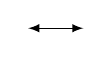
\begin{tikzpicture}[scale=0.7]
    \def\Radius{.09}
    \LagrangeCell{-4}{0}{2}{\Radius}{1}{{,,,}};
    
    \draw[>=latex, <->] (-1.5,1) -- (-.5,1);
    
    \LagrangeCell{0}{0}{1}{\Radius}{1}{{,,,}};
    \LagrangeCell{0}{1}{1}{\Radius}{1}{{,,,}};
    \LagrangeCell{1}{0}{1}{\Radius}{1}{{,,,}};
    \LagrangeCell{1}{1}{1}{\Radius}{1}{{,,,}};
    \end{tikzpicture}
    \caption{\h-adaptation}
  \end{figure}
\end{minipage}

\begin{table}
\caption{Error prediction algorithm based on \parencite{melenk2001}}
\vspace{-1em}
\begin{tabular}{ll}
  \rowcolor{fzjblue!25} \multicolumn{1}{c}{\textbf{Adaptation type}} & \multicolumn{1}{c}{\textbf{Prediction formula}} \\
  \toprule
  no adaptation & $\eta_{K,\text{pred}} = \eta_{K} \, \gamma_\text{n}$ \\
  \midrule
  \p-adaptation & $\eta_{K,\text{pred}} = \eta_{K} \,
\gamma_\text{p}^{(p_{K,\text{future}} - p_K)}$ \\
  \midrule
  \hp-refinement & $\left( \eta_{K_c,\text{pred}} \right)^2 = n_{K_c}^{-1}
\left( \eta_{K_p} \,
\gamma_\text{h} \, 0.5^{p_{K_c,\text{future}}} \,
\gamma_\text{p}^{(p_{K_c,\text{future}} - p_{K_p})} \right)^2$ \\
  \addlinespace[1mm]
  \hp-coarsening & $\left( \eta_{K_p,\text{pred}} \right)^2 = \sum\limits_{K_c} \left( \eta_{K_c} \,
(\gamma_\text{h} \, 0.5^{p_{K_p,\text{future}}})^{-1} \, \gamma_\text{p}^{(p_{K_p,\text{future}} - p_{K_c})} \right)^2$
\end{tabular}
\end{table}
\end{frame}





\begin{frame}
\frametitle{Smoothness estimation}

\begin{itemize}
\item Different representations of finite element approximation
\begin{align*}
u_{hp}(x) = \sum\limits_i u_i \, \varphi_i(x)  = \sum\limits_k c_k \, P_k(x)
\end{align*}
\end{itemize}

\begin{itemize}
\item Choose orthogonal basis $\{P_k\}$ of increasing frequency
\item Uniquely attribute frequency of oscillations to each basis function
\end{itemize}
\end{frame}





\begin{frame}
\frametitle{Orthogonal basis}

\begin{itemize}
\item Legendre: Orthogonal basis of polynomials
  \begin{align*}
  P_k(x) &= \frac{1}{2^k k!} \frac{d^k}{dx^k} \left( (x^2 - 1)^k \right) \\
  \langle P_k, P_l \rangle &= \int P_k(x) \, P_l(x) \, dx = \frac{2}{2k+1} \delta_{kl}
  \end{align*}
\end{itemize}

\begin{itemize}
\item Fourier: Orthogonal basis of sinusoids
  \begin{align*}
  P_k(x) &= \exp \left( -i \, 2 \pi k \, x \right) \\
  \langle P_k, P_l \rangle &= \int P_k(x) \, P_l^*(x) \, dx = \delta_{kl}
  \end{align*}
\end{itemize}
\end{frame}





\begin{frame}
\frametitle{Legendre polynomials}

\begin{tikzpicture}
\begin{axis}[
%cycle list/Dark2,
scale=.97,
ymin=-1.2, ymax=1.2,
xlabel=$x$,
ylabel=$P_k(x)$,
grid=major,
%legend style={at={(0.5,1.02)}, anchor=south, /tikz/every even column/.append style={column sep=0.5cm}},
%legend columns=3,
legend cell align=left,
legend pos = outer north east,
legend style={font=\tiny},
cycle list/Dark2,
every axis plot/.append style={ultra thick}
]
\addplot+[samples=2, domain=-1:1] {1};
\addlegendentry{$P_0 = 1$};

\only<2->{
\addplot+[samples=2, domain=-1:1] {x};
\addlegendentry{$P_1 = x$};
}

\only<3->{
\addplot+[samples=20, domain=-1:1] {0.5*(3*x^2-1)};
\addlegendentry{$P_2 = \frac{1}{2} \left( 3x^2 - 1 \right)$};
}

\only<4->{
\addplot+[samples=40, domain=-1:1] {0.5*(5*x^3 - 3*x)};
\addlegendentry{$P_3 = \frac{1}{2} \left( 5x^3 - 3x \right)$};
}

\only<5->{
\addplot+[samples=60, domain=-1:1] {0.125*(35*x^4 - 30*x^2 + 3)};
\addlegendentry{$P_4 = \frac{1}{8} \left( 35x^4 - 30x^2 + 3 \right)$};
}

\only<6->{
\addplot+[samples=80, domain=-1:1] {0.125*(63*x^5 - 70*x^3 + 15*x)};
\addlegendentry{$P_5 = \frac{1}{8} \left( 63x^5 - 70x^3 + 15x \right)$};
}
\end{axis}
\end{tikzpicture}
\end{frame}





\begin{frame}
\frametitle{Fourier sinusoids}

\begin{tikzpicture}
\begin{axis}[
%cycle list/Dark2,
scale=.97,
ymin=-1.2, ymax=1.2,
xlabel=$x$,
ylabel=$\operatorname{Re}\left(P_k(x)\right)$,
grid=major,
%legend style={at={(0.5,1.02)}, anchor=south, /tikz/every even column/.append style={column sep=0.5cm}},
%legend columns=3,
legend cell align=left,
legend pos = outer north east,
legend style={font=\tiny},
cycle list/Dark2,
every axis plot/.append style={ultra thick}
]
\addplot+[samples=2, domain=0:1] {1};
\addlegendentry{$P_0 = 1$};

\only<2->{
\addplot+[samples=30, domain=0:1] {cos(deg(6.28*x))};
\addlegendentry{$P_1 = \exp\left(i \, 2\pi \, x\right)$};
}

\only<3->{
\addplot+[samples=60, domain=0:1] {cos(deg(2*6.28*x))};
\addlegendentry{$P_2 = \exp\left(i \, 4\pi \, x\right)$};
}

\only<4->{
\addplot+[samples=90, domain=0:1] {cos(deg(3*6.28*x))};
\addlegendentry{$P_3 = \exp\left(i \, 6\pi \, x\right)$};
}

\only<5->{
\addplot+[samples=120, domain=0:1] {cos(deg(4*6.28*x))};
\addlegendentry{$P_4 = \exp\left(i \, 8\pi \, x\right)$};
}
\end{axis}
\end{tikzpicture}
\end{frame}





\begin{frame}
\frametitle{Decay of Legendre coefficients}

\begin{itemize}
\item Determine coefficients $\{c_k\}$ on every cell $K$:
  \begin{align*}
  c_k = \int\limits_K u_{hp}(x) \, P_k(x) \, dx
  \end{align*}
  
\item FE approximation is analytic if coefficients decay exponentially \cite{eibner2007}
  \begin{align*}
  |c_k| \leq C \exp\left( - \sigma |k| \right)
  \end{align*}
  
\item Determine decay rate $\sigma$ via least-squares fit
  \begin{align*}
  \ln(|c_k|) \sim \tilde{C} - \sigma |k|
  \end{align*}
\end{itemize}

\vspace{-1em}
\begin{block}{\vspace{-1em}}
\centering
Decay rates $\sigma$ considered as smoothness estimates \\
Keep $p$ large if $\sigma$ is large
\end{block}
\vspace{1em}
\end{frame}





\begin{frame}
\frametitle{Decay of Fourier coefficients}

\begin{itemize}
\item FE approximation is part of Hilbert space $\mathcal{H}^s$ if integral exists
  \begin{align*}
  \int\limits_K \left| \nabla^s u_{\text{hp}}(x) \right|^2 dx &= (2 \pi)^{2s} \sum\limits_k \left| c_k \right|^2 k^{2s} < \infty \\
  \Rightarrow\qquad |c_k| = \mathcal{O}&\left(k^{-\sigma - \epsilon}\right)  \quad \text{with} \quad \sigma = s + \text{dim}/2
  \end{align*}

\item Determine coefficients $\{c_k\}$ and their decay via least-squares fit on every cell $K$:
  \begin{align*}
  c_k &= \int\limits_K u_{hp}(x) \, P_k^*(x) \, dx & \ln(|c_k|) &\sim C - \sigma \ln\left( |k| \right)
  \end{align*}
\end{itemize}

\vspace{-1em}
\begin{block}{\vspace{-1em}}
\centering
Decay rates $\sigma$ considered as smoothness estimates \\
Keep $p$ large if $\sigma$ is large
\end{block}
\vspace{1em}
\end{frame}

\subtitle{More results}
\maketitle
\section{Error versus performance}
\label{sec:errorvsperformance}

%Global H1 error as measure
%\begin{align}
%\| e_{hp} \|_{H^1(\Omega)}^2 &= \sum\limits_K \| e_{hp} (\vec{x}) \|_{H^1(K)}^2 \\
%\| e_{hp} \|_{H^1(K)}^2 &= \int_K (|e_{hp}|^2 + |\nabla e_{hp}|^2) \differential{\vec{x}}
%\end{align}
%with error function $e_{hp} = u - u_{hp}$.

% setup of scenario

The main motivation of \hp-adaptive methods are their superior error convergence characteristics compared to the more common \h-adaptive ones provided that the solution is sufficiently regular. We will demonstrate their advantages on our presented scenario and use consecutively adapted meshes to illustrate their error performance in relation to their workload on the numerical example.

%Demonstrate adaptive algorithms , and how the error reduces with.
%compare error with the workload either measured in the number of \glspl{dof} or the actual wall time. % maybe later

The consecutively adapted meshes so created are by far not optimal for the problem, nor is finding such an optimal mesh subject of this dissertation. We are rather interested in comparing the performance and results of the decision algorithms presented in Sec.~\ref{sec:decision}, and whether they are capable of localizing regions with singularities, i.e.\@ the one at the point of origin for our numerical example. We will compare all types of adaptation at our disposal, i.e.\@ \h-, \p-, and \hp-adaptation. For the latter, we examine all three presented strategies in contrast, namely error prediction and smoothness estimation by either Legendre or Fourier coefficient decay.

After solving the linear equation system in each step and calculating the error on basis of the analytic solution according to \textcite{kelly1983}, we use the \textit{fixed-number} strategy to indicate adaptation: The 30\% fraction of all cells with the highest error will be flagged for refinement, and 3\% of those with the lowest error will be marked for coarsening. This allows us to compare the results of each adaptation type under the same conditions, since always the same amount of cells is going to be changed. The idea behind additional coarsening is motivated by the fact that we tend to refine too many cells with error estimators providing an upper bound for the error, or error indicators based on heuristics. We would like to correct this from a previous iteration by coarsening a small amount of cells. The combination of fractions of 30\% for refinement and 3\% for coarsening has become a reasonable choice for two-dimensional applications within the \dealii{} library.

%We will compared different refinement strategies. We will use \textit{fixed-fraction} adaptation so that every cell is refined. This allows us to compare the choices of all strategies since always the same amount of cells is taken into account. \todo{see slack text}

Further for \hp-adaptive strategies, we need to choose a decision strategy providing corresponding indicators that propose which type of adaptation we want to impose one each cell.
%
Again, we use the \textit{fixed-number} algorithm on all decision indicators. This allows us to compare the choices made by each strategy since always the same amount of cells is going to be changed in terms of both \h- and \p-adaptation, respectively.
%
As a first naive approach, we will impose the \h-variant on one half of all cells previously marked for adaptation, and the \p-variant on the other half.
%As a first naive approach, we choose between \h- and \p-adaptation fifty fifty among all cells that have been previously marked for adaptation.
%, based on the specified decision criterion.
As a second attempt, since we know that we have only one single localized and well-defined singularity in the domain, we are confident to make an educated guess and assign 90\% of flagged cells for \p- and the remaining 10\% for \h-adaptation. From here, we refer to the first approach if we call a decision strategy naive, and speak of the second if no such attribute was given.

To setup the numerical example, we start with a mesh consisting of three cells as the coarsest possible representation of our L-shaped domain, which will be globally refined five times to form the initial grid for all investigations in this section.

The error prediction strategy forms an exception since it requires a prepended initialization step. In this case, we will begin with four initial refinement steps, solve the equation system, and perform another global refinement so that we have the corresponding prediction available. Further for this strategy, control parameters are set to $\gamma_n = 1$, $\gamma_h = 1$, and $\gamma_p = \sqrt{0.4}$, which corresponds to the values used by \textcites{melenk2001}{mitchell2014}.

We use a collection of Lagrangian finite elements $Q_p$ with polynomial degrees $p \in [2,7]$ and skip linear elements due to our observation that the smoothness estimation algorithms perform poorly with those. All cells will be initially assigned with the lowest order element. In the case of sole \h-adaptation, all elements will be assigned to $Q_2$ elements. For pure \p-adaptation, we favor \p-adaptation to \h-adaptation as long as the finite element can be \p-adapted, i.e.\@ the current finite element is neither at the top nor the bottom of the hierarchy. We perform a total of twelve consecutive adaptation iterations, so twice as many as there are different finite elements.

All calculations in this section have been carried out on a desktop machine, using an Intel \todo{trademark} Core i7-4790 processor running at 3.6 GHz with 32 GB of memory \todo{si}. Although this is a quad-core processor offering a total of eight threads utilizing hypertreading, we will only use a single thread for our calculations, which is sufficient to determine both error and workload. We will deal with parallelization in later sections.


% results: error vs ndofs

Representatively, we will show the grid and distribution of finite elements after six adaptation cycles of the Legendre coefficient decay strategy with the educated guess approach in Fig.~\ref{fig:fedegrees}. All other meshes after equally many adaptation iterations from the other strategies are showcased in App.~\ref{app::strategies}.

We see that the Legendre strategy is able to locate the singularity in the center by preferring \h-adaptive refinement in this section, while using \p-adaptation in the other regions. This is also the case for all other strategies, naiive or not, as shown in App.~\ref{app::strategies}.

\begin{figure}
\centering
Insert distribution of finite elements for Legendre strategy after five iterations.
\caption{Distribution of finite elements after five iterations with the Legendre coefficient decay strategy.}
\label{fig:fedegrees}
\end{figure}

We will plot the $H_1$ error against the workload, which can be measured in two ways: Either with the number of \glspl{dof}, or the elapsed real time from start to end of our application, which we refer to as wall time. We begin with identifying the workload with the former and show corresponding results in Fig.~\ref{fig:errordofs}.

%We measure the workload in two different ways and present the results separately. First, with the number of \glspl{dof} for each individual iteration, and second, with the total wall time accumulated over the current and all previous iterations.

\begin{figure}
\begin{subfigure}{1\textwidth}
  \centering
  \begin{tikzpicture}
\begin{loglogaxis}[
  xlabel=Number of \glspl{dof},
  ylabel=H1 error]
\addplot table [y=H1 error, x=ndofs, col sep=comma] {data/error/h.csv};
\addplot table [y=H1 error, x=ndofs, col sep=comma] {data/error/p.csv};
\addplot table [y=H1 error, x=ndofs, col sep=comma] {data/error/hp-legendre.csv};
\addplot table [y=H1 error, x=ndofs, col sep=comma] {data/error/hp-fourier.csv};
\addplot table [y=H1 error, x=ndofs, col sep=comma] {data/error/hp-prediction.csv};
\addplot table [y=H1 error, x=ndofs, col sep=comma] {data/error/hp-legendre-naive.csv};
\addplot table [y=H1 error, x=ndofs, col sep=comma] {data/error/hp-fourier-naive.csv};
\addplot table [y=H1 error, x=ndofs, col sep=comma] {data/error/hp-prediction-naive.csv};
\end{loglogaxis}
\end{tikzpicture}
  \caption{Double logarithmic representation. The thick line corresponds to the reference Eq.~(\ref{eq:errorbound_ana}).}
  \label{fig:errordofsloglog}
\end{subfigure}
\begin{subfigure}{1\textwidth}
  \centering
  \begin{tikzpicture}
\begin{semilogyaxis}[
%  scale only axis,
  xlabel=Number of \glspl{dof},
  ylabel=H1 error,
  legend pos=outer north east]
%\addplot table [y=H1 error, x=ndofs, col sep=comma] {data/error/h.csv};
%\addlegendentry{\h};

\addplot table [y=H1 error, x=ndofs, col sep=comma, select coords between index={0}{5}] {data/error/p.csv};
\addlegendentry{\p};

\addplot table [y=H1 error, x=ndofs, col sep=comma, select coords between index={0}{5}] {data/error/hp-legendre.csv};
\addlegendentry{\hp{}-Legendre};

\addplot table [y=H1 error, x=ndofs, col sep=comma, select coords between index={0}{5}] {data/error/hp-fourier.csv};
\addlegendentry{\hp{}-Fourier};

\addplot table [y=H1 error, x=ndofs, col sep=comma, select coords between index={0}{6}] {data/error/hp-prediction.csv};
\addlegendentry{\hp{}-prediction};

%\addplot table [y=H1 error, x=ndofs, col sep=comma] {data/error/hp-legendre-naive.csv};
%\addlegendentry{\hp{}-Legendre naive};
%
%\addplot table [y=H1 error, x=ndofs, col sep=comma] {data/error/hp-fourier-naive.csv};
%\addlegendentry{\hp{}-Fourier naive};
%
%\addplot table [y=H1 error, x=ndofs, col sep=comma] {data/error/hp-prediction-naive.csv};
%\addlegendentry{\hp{}-prediction naive};

%\addplot[very thick, samples=100, domain=10000:50000] {10^(-2)*exp(10^(-3.9)*(-x+10000))}; % {10^(-4)*(-x+10000)};
\end{semilogyaxis}
\end{tikzpicture}
  \caption{Customly scaled coordinate system with the y-axis scaled exponentially and the x-axis scaled with the cubic root. The thick line corresponds to the reference Eq.~(\ref{eq:errorbound_exp}) with $b = 0.18$.}
  \label{fig:errordofscustom}
\end{subfigure}
\caption{Error vs workload.}
\label{fig:errordofs}
\end{figure}

The double logarithmic representation of our results in Fig.~\ref{fig:errordofsloglog} reveals analytic convergence for the \h-adaptive case, but at a lower rate as presented in Eq.~(\ref{eq:errorbound_ana}), which translates to $n_\text{dofs}^{-1}$ in our scenario. An explanation would be that we are not working with quasiuniform but rather highly adapted meshes.

Eq.~(\ref{eq:errorbound_exp}) predicts exponential decay for \hp-adaptive strategies, which we would like to verify in Fig.~\ref{fig:errordofscustom} with a customly scaled plot featuring a logarithmic y-axis and an x-axis scaled with the cubic root, which corresponds to the correct exponent in our numerical example. Indeed, we see exponential convergence in the \p-adaptive and \hp-adaptive strategies to the proclaimed rate, however the naive approaches miss it. Thus a high proportion of \p-refinement is required to yield exponential decay in this scenario.

The \p-strategy shows a similar decay as the \hp-adaptive methods.%, but the error in the last cycle is still by a factor of two higher.
In this strategy, \p-refinement will be applied up to the point until it is no longer possible after we reached the highest order element in the hierarchy. With six distinct finite elements in our collection, we will apply \h-refinement for the first time after the sixth data point, at which a major drop is observable. We also see that the exponential decay proclaimed in Eq.~(\ref{eq:errorbound_exp}) is only observable after applying \h-refinement. Thus, we conclude that \h-refinement is mandatory to reduce the error to the observed low order of magnitude.

To solve the equation system in the last adaptation cycle, the \hp-adaptive methods %corresponding to our educated guess 
srequire a number of \glspl{dof} by a factor of 100 less than the \h-adaptive methods to reach the same accuracy
%need a factor of 1,000 less \gls{dof} to reach the same accuracy as the \h-adaptive methods
and by factor of 10 less compared to their naive counterparts. This demonstrates that \hp-adaptive methods are the methods of choice for this particular scenario.

%We conclude that \p-heavy refinement combined with \h-adaptation near the singularity perform the best error per workload ratio.

In the course of adaptation with the Fourier strategy, some adaptation steps increase the number of \gls{dof} without decreasing the error, which we refer to as 'hickups'.
%We see certain outliers in the plots for Fourier strategy.
We observed that they occur if the finite element with the highest polynomial degree in our mesh increases from fourth to fifth order. This is perhaps not a causal relation, and we have not yet found the reason for these 'hickups'.

%Compared to \h- and naive \hp-approaches, \p- and \hp-strategies featuring the educated guess yield similar results.

%We reach about one order of magnitude lower errors with \hp-adaptive strategies compared to the \p-adaptive, which might be due to the singularity that the latter does not resolve \todo{?}.


% results: error vs walltime

From a practical point of view, the error performance will now be compared to the actual wall time to measure whether we have an economic benefit in using \hp-adaptive methods. For each consecutive adaptation cycle, we again plot the calculated error against the workload, which is this time represented by the total run time accumulated over the current and all previous iterations. Each run will be repeated five times and the minimum over the total runtime over all runs will be picked to compensate for temporarily high loads on memory bandwidth. The results are shown in Fig.~\ref{fig:errorwalltime}.

\begin{figure}
%\begin{subfigure}{1\textwidth}
\centering
\begin{tikzpicture}
\begin{loglogaxis}[
  xlabel=Wall time {[seconds]},
  ylabel=H1 error,
  legend pos=outer north east]
\addplot table [y=H1 error, x=walltime, col sep=comma] {data/error/h.csv};
\addlegendentry{\h};

\addplot table [y=H1 error, x=walltime, col sep=comma] {data/error/p.csv};
\addlegendentry{\p};

\addplot table [y=H1 error, x=walltime, col sep=comma] {data/error/hp-legendre.csv};
\addlegendentry{\hp{}-Legendre};

\addplot table [y=H1 error, x=walltime, col sep=comma] {data/error/hp-fourier.csv};
\addlegendentry{\hp{}-Fourier};

\addplot table [y=H1 error, x=walltime, col sep=comma] {data/error/hp-prediction.csv};
\addlegendentry{\hp{}-prediction};

\addplot table [y=H1 error, x=walltime, col sep=comma] {data/error/hp-legendre-naive.csv};
\addlegendentry{\hp{}-Legendre naive};

\addplot table [y=H1 error, x=walltime, col sep=comma] {data/error/hp-fourier-naive.csv};
\addlegendentry{\hp{}-Fourier naive};

\addplot table [y=H1 error, x=walltime, col sep=comma] {data/error/hp-prediction-naive.csv};
\addlegendentry{\hp{}-prediction naive};
\end{loglogaxis}
\end{tikzpicture}
%  \caption{Error vs workload.}
%  \label{fig:errorexpworkload}
%\end{subfigure}
%\begin{subfigure}{1\textwidth}
%  \centering
%  \begin{tikzpicture}
\begin{semilogyaxis}[
  xlabel=Wall time {[seconds]},
  ylabel=H1 error,
  legend pos=outer north east]
%\addplot table [y=H1 error, x=walltime, col sep=comma] {data/error/h.csv};
%\addlegendentry{\h};

\addplot table [y=H1 error, x=walltime, col sep=comma, select coords between index={0}{5}] {data/error/p.csv};
\addlegendentry{\p};

\addplot table [y=H1 error, x=walltime, col sep=comma, select coords between index={0}{5}] {data/error/hp-legendre.csv};
\addlegendentry{\hp{}-Legendre};

\addplot table [y=H1 error, x=walltime, col sep=comma, select coords between index={0}{5}] {data/error/hp-fourier.csv};
\addlegendentry{\hp{}-Fourier};

\addplot table [y=H1 error, x=walltime, col sep=comma, select coords between index={0}{6}] {data/error/hp-prediction.csv};
\addlegendentry{\hp{}-prediction};

%\addplot table [y=H1 error, x=walltime, col sep=comma] {data/error/hp-legendre-naive.csv};
%\addlegendentry{\hp{}-Legendre naive};
%
%\addplot table [y=H1 error, x=walltime, col sep=comma] {data/error/hp-fourier-naive.csv};
%\addlegendentry{\hp{}-Fourier naive};
%
%\addplot table [y=H1 error, x=walltime, col sep=comma] {data/error/hp-prediction-naive.csv};
%\addlegendentry{\hp{}-prediction naive};

%\addplot[very thick, samples=100, domain=0.1:5] {10^(-2)*exp(10^(0)*(-x+0.1))}; % {10^(-4)*(-x+10000)};
\end{semilogyaxis}
\end{tikzpicture}
%  \caption{Error vs walltime.}
%  \label{fig:errorexpwalltime}
%\end{subfigure}
\caption{Double lagarithmic error vs walltime.}
\label{fig:errorwalltime}
\end{figure}

%We notice that the choice of the \hp-adaptive strategy has an impact on the error performance compared to the number of \glspl{dof}. However in comparing error with the runtime, we see that all methods perform similarly. We will postpone the discussion on this topic for the later Sec.~() in which we give an in-depth analysis on the sacalability of certain parts of our code, in which we think to identify the reason for this behavior.

Again after the last adaptation cycle, \p- and \hp-adaptive methods are most efficient and about an order of magnitude faster than the \h-adaptive variant. Interestingly, the wall times of the naive \hp-strategies fan out. It appears that a high diversity of finite elements compared with major grid adaptation increase the wall time significantly, and we suspect that the combination of solver and \gls{amg} preconditioner is responsible for this behavior. We will discuss this topic later in the scalability analysis.

The Fourier strategy takes the longest wall time for initialization, during which the Fourier transformation matrices are calculated. This is a costly operation, which requires substantially more quadrature points during calculation than the Legendre equivalent, and is responsible for the observable offset.

% this is general observation
Among all \hp-strategies of either naive or educated guess category, we do not see major differences in their performance, but overall the Legendre coefficient decay strategy stands out in both categories with the best error per workload performance in either way workload is defined.
%Compared to the Fourier strategy, it seems to be better suited for \gls{fem} since its basis functions are also based on polynomials.

% write this in the next chaper
%In the upcoming scalability analysis, we will thus pick this strategy with Legendre coefficient and the educated guess.

%Overall, the Legendre coefficient strategy yields the best error per workload performance in both categories.

%Again, to mitigate the impact of temporary slowdowns on the supercomputer due to a high loads on memory and network bandwidth, we repeat each run for a total of \todo{five?} times and take the minimal runtime in each category over all runs.
\section{Load balancing heuristics}
\label{sec:heuristics}

% introduction

For parallel computations on distributed memory systems, the global domain is partitioned into several subdomains, each of which is assigned to a single process. Such a mesh decomposition is showcased in Fig.~\ref{fig:decomposition}.

\begin{figure}
\centering
\begin{subfigure}[t]{.49\textwidth}
  \centering
  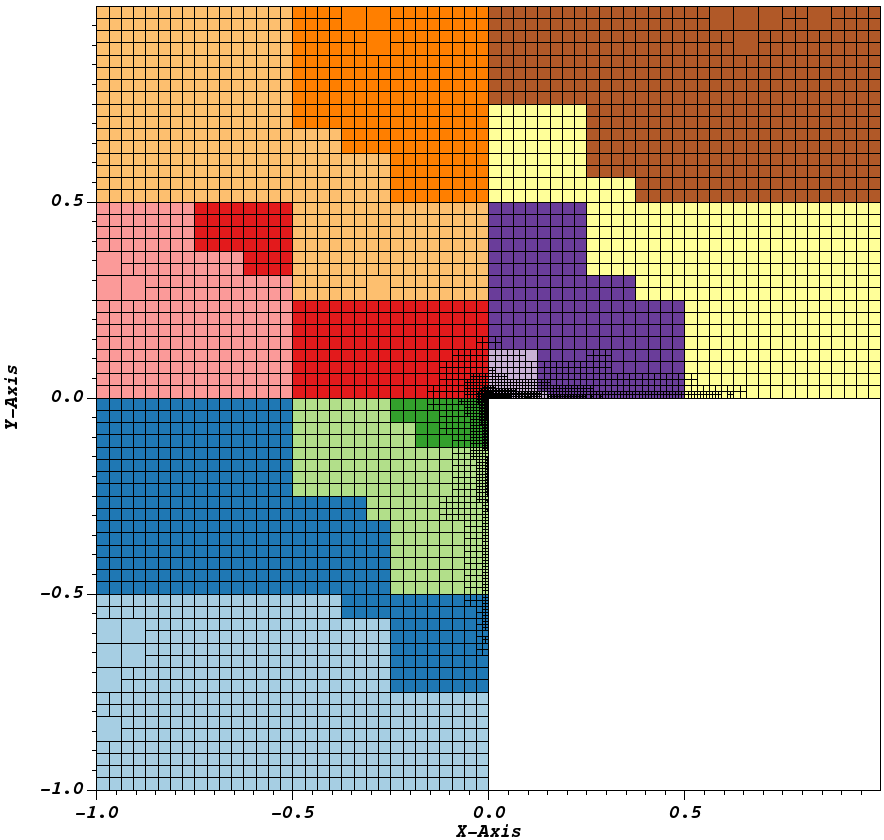
\includegraphics[width=\textwidth]{figures/results/corner-2d-error-hp-legendre-05_subdomain12.png}
  \caption{Constant weighting.}
\end{subfigure}
\begin{subfigure}[t]{.49\textwidth}
  \centering
  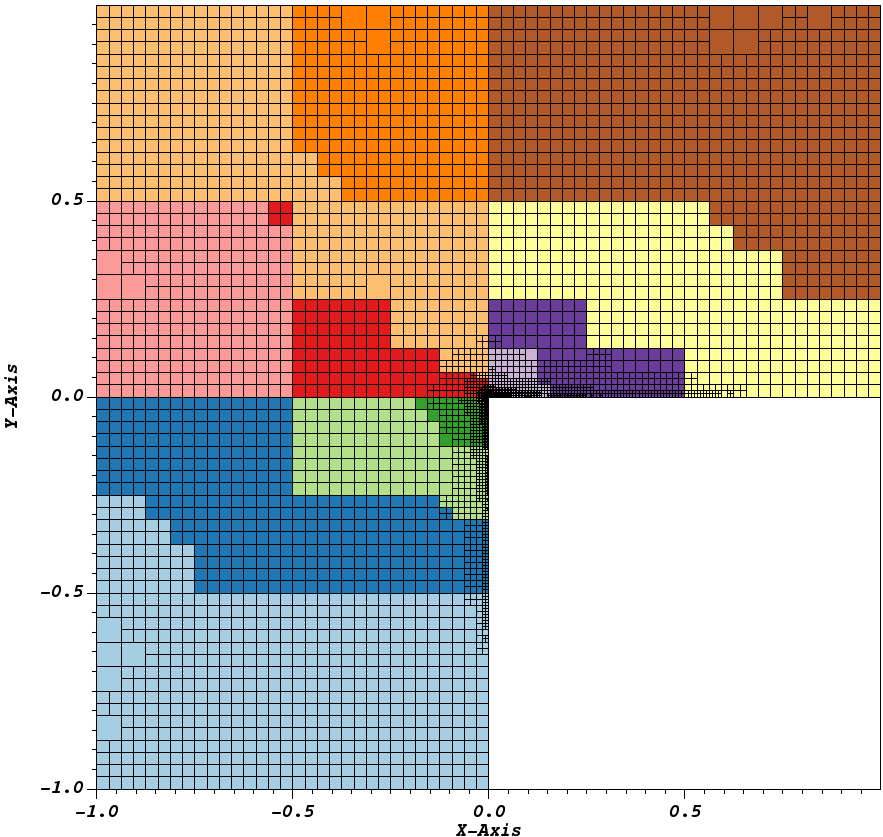
\includegraphics[width=\textwidth]{figures/results/corner-2d-error-hp-legendre-05_subdomain12_customweighting.png}
  \caption{Weighting with an individually potentiated number of \glspl{dof}, i.e.\@ $\propto n_\text{dofs}^{1.9}$.}
\end{subfigure}
\caption{Decomposition of the mesh after six iterations with the Legendre coefficient decay strategy on 12 \gls{mpi} processes with various cell weighting. Each color represents a different subdomain.}
\label{fig:decomposition}
\end{figure}

Proper load balancing is necessary for an efficient use of all computational resources. Especially on \gls{hpc} systems with lots of available processors, this is a critical feature. For \hp-adaptive \gls{fem}, we presented approaches for load balancing in Sec.~\ref{sec:loadbalancing} by assigning weights to each individual cell and balancing the accumulated weight among all processes. We relate the weight to the number of \glspl{dof} on each cell potentiated by an exponent that we will determine in the upcoming investigations. Or in other words, cell weights are chosen proportional to $n_\text{dofs}^c$ with the exponent $c$ to be ascertained.

Although all three \hp-adaptive strategies have demonstrated a similar performance as shown in Sec.~\ref{sec:errorvsperformance}, we pick only one adaptation strategy for our parallel investigations. We choose the smoothness estimation strategy based on the decay of Legendre coefficients as the most efficient one for this purpose.

% system specifications

Investigations are carried out on the JURECA supercomputer \parencite{krause2016}. Each computing node is equipped with two Intel\textsuperscript{\textregistered} Xeon\textsuperscript{\textregistered} E5-2680 v3 processors with twelve cores running at 2.5GHz and either 128GB, 256GB or 512GB of memory. With simultaneous multithreading, a total of 48 threads are available per node. Communication between nodes happens via a Mellanox EDR InfiniBand high-speed network.

In this section, our investigations are performed on two distinct nodes, which provide a total of 96 threads and involve communication between two physically independent memory segments. We expect that this setup yields representative results that can be extrapolated on even larger problem sizes.

Further, we use a 'flat' \gls{mpi} model: Every thread will be assigned to an individual \gls{mpi} process and no additional thread parallelization is invoked. Although \dealii{} provides such a feature via Intel\textsuperscript{\textregistered} \gls{tbb}, we refrain from using it to measure the pure \gls{mpi} performance for all parallel analyses in this dissertation.

% problem specifications

To qualify our problem for parallel computations, we need to increase its size drastically. The problem is initialized with nine global refinements and gets adapted in twelve iterations. For the strategy with the Legendre coefficient decay, this results in a total number of 46,369,440 \glspl{dof}, so that in the best case each process will be assigned to a number of 483,015 \glspl{dof} on average. Each type of finite element from the provided collection is represented at least once in the mesh.

This advanced scenario will form the basis of our investigations to see how different weighting exponents affect the wall time, and which one provides a minimum. With serialization, we ensure that each of these runs conforms to the same conditions. Again, to mitigate the impact of temporary slowdowns on the supercomputer due to high loads on memory and network bandwidth, we repeat each run for a total of five times and take the minimum wall time in each category over all runs.

% results

For varying weighting exponents, we compare the wall times of the full adaptation cycle and its relevant sections
%For resumed scenarios in which the mesh will be partitioned according to weights with different weighting exponents, we compare the wall time of critical sections of the program as well as the total wall time
%between runs with different weighting exponents
in Fig.~\ref{fig:weights}.

\todo{Second scale for assembly/discontinued axis with groupplot}
%https://tex.stackexchange.com/questions/46422/axis-break-in-pgfplots
\todo{Maybe also add setup of data structure and other parts}
\begin{figure}
\centering
\begin{tikzpicture}
\begin{axis}[
  xlabel=Weighting exponent,
  ylabel=Wall time {[seconds]},
  legend pos=outer north east]

\addplot table [y=full cycle, x=weighting exponent, col sep=comma] {data/weight/weight.csv};
\addlegendentry{full cycle};

\addplot table [y=assembly, x=weighting exponent, col sep=comma] {data/weight/weight.csv};
\addlegendentry{assemble linear system};

\addplot table [y=solve, x=weighting exponent, col sep=comma] {data/weight/weight.csv};
\addlegendentry{linear solver and preconditioner};
\end{axis}
\end{tikzpicture}
\caption[Wall times for load balancing with varying weighting exponents.]{Wall times of a complete adaptation cycle and those parts relevant for load balancing. The problem has a number of about 46 million \glspl{dof} and is solved on 2 nodes or 96 \gls{mpi} processes. Weights proportional to $n_\text{dofs}^c$ will be assigned to each cell with varying exponents $c$.}
\label{fig:weights}
\end{figure}

As discussed in Sec.~\ref{sec:balancing}, the assembly of the equation system and the its solution are identified as the critical sections whose wall time is affected by the number of \glspl{dof}. We see that the solution of the equation system takes about 90\% of the total wall time and is the crucial factor for proper load balancing. The minimal wall time for both solver and the full cycle is reached with a weighting exponent of $c = 1.9$.

We were surprised to find the minimum wall time of the solver at such a high exponent, since we expected $c = 1$ for an efficient solver. This may be related to the implementation of the preconditioner combined with the disorder that \hp-adaptive methods cause in the system matrix. Further, we were expecting a minimum in the assembly at about $c = 2$, but found it was decaying at even higher exponents. We have no explanation for this behavior. Analyzing the effect of cell weighting on each individual section of the program
%the load balancing
will be subject of further investigations.

% Next step
%We set an weighting expoenent to a value of $c = 1.9$ for the following considerations regarding scalability.

\begin{frame}
\frametitle{Scaling on successive refinement}

\begin{figure}
\hspace*{-0.5em}
\begin{tikzpicture}
\begin{loglogaxis}[
scale=0.9,
xlabel={Number of degrees of freedom},
ylabel={Wall time [seconds]},
grid=major,
legend cell align=left,
legend pos=outer north east,
legend style={font=\tiny}
]

% data
\addplot table [y=solve, x=ndofs, col sep=comma] {data/weak/weak-nodes16.csv};
\addlegendentry{linear solver};

\addplot table [y=setup, x=ndofs, col sep=comma] {data/weak/weak-nodes16.csv};
\addlegendentry{setup data structures};

\addplot table [y=assembly, x=ndofs, col sep=comma] {data/weak/weak-nodes16.csv};
\addlegendentry{assemble linear system};

\addplot table [y=compute errors, x=ndofs, col sep=comma] {data/weak/weak-nodes16.csv};
\addlegendentry{estimate error};

\addplot table [y=calculate indicators, x=ndofs, col sep=comma] {data/weak/weak-nodes16.csv};
\addlegendentry{estimate smoothness};

\addplot table [y=refine, x=ndofs, col sep=comma] {data/weak/weak-nodes16.csv};
\addlegendentry{coarsen and refine};

% optimal line
\addplot[very thick, samples=2, domain=12591105:1302365268] {10^(-7.2)*x};
\addlegendentry{optimal convergence};

% auxiliary lines
\begin{scope}
\draw[green, very thick] ({axis cs:76800000,0}|-{rel axis cs:0,1}) -- ({axis cs:76800000,0}|-{rel axis cs:0,0});
\draw[blue, very thick] ({axis cs:50647318,0}|-{rel axis cs:0,1}) -- ({axis cs:50647318,0}|-{rel axis cs:0,0});
\end{scope}
\addlegendimage{color=green};
\addlegendentry{$10^5$ DoFs per process};
\addlegendimage{color=blue};
\addlegendentry{each reference finite element in mesh};
\end{loglogaxis}
\end{tikzpicture}
\caption{Scaling on successively refined grids}
\end{figure}
\end{frame}

\end{document}
